% Options for packages loaded elsewhere
\PassOptionsToPackage{unicode}{hyperref}
\PassOptionsToPackage{hyphens}{url}
\PassOptionsToPackage{dvipsnames,svgnames,x11names}{xcolor}
%
\documentclass[
  letterpaper,
  DIV=11,
  numbers=noendperiod]{scrartcl}

\usepackage{amsmath,amssymb}
\usepackage{iftex}
\ifPDFTeX
  \usepackage[T1]{fontenc}
  \usepackage[utf8]{inputenc}
  \usepackage{textcomp} % provide euro and other symbols
\else % if luatex or xetex
  \usepackage{unicode-math}
  \defaultfontfeatures{Scale=MatchLowercase}
  \defaultfontfeatures[\rmfamily]{Ligatures=TeX,Scale=1}
\fi
\usepackage{lmodern}
\ifPDFTeX\else  
    % xetex/luatex font selection
\fi
% Use upquote if available, for straight quotes in verbatim environments
\IfFileExists{upquote.sty}{\usepackage{upquote}}{}
\IfFileExists{microtype.sty}{% use microtype if available
  \usepackage[]{microtype}
  \UseMicrotypeSet[protrusion]{basicmath} % disable protrusion for tt fonts
}{}
\makeatletter
\@ifundefined{KOMAClassName}{% if non-KOMA class
  \IfFileExists{parskip.sty}{%
    \usepackage{parskip}
  }{% else
    \setlength{\parindent}{0pt}
    \setlength{\parskip}{6pt plus 2pt minus 1pt}}
}{% if KOMA class
  \KOMAoptions{parskip=half}}
\makeatother
\usepackage{xcolor}
\setlength{\emergencystretch}{3em} % prevent overfull lines
\setcounter{secnumdepth}{-\maxdimen} % remove section numbering
% Make \paragraph and \subparagraph free-standing
\ifx\paragraph\undefined\else
  \let\oldparagraph\paragraph
  \renewcommand{\paragraph}[1]{\oldparagraph{#1}\mbox{}}
\fi
\ifx\subparagraph\undefined\else
  \let\oldsubparagraph\subparagraph
  \renewcommand{\subparagraph}[1]{\oldsubparagraph{#1}\mbox{}}
\fi


\providecommand{\tightlist}{%
  \setlength{\itemsep}{0pt}\setlength{\parskip}{0pt}}\usepackage{longtable,booktabs,array}
\usepackage{calc} % for calculating minipage widths
% Correct order of tables after \paragraph or \subparagraph
\usepackage{etoolbox}
\makeatletter
\patchcmd\longtable{\par}{\if@noskipsec\mbox{}\fi\par}{}{}
\makeatother
% Allow footnotes in longtable head/foot
\IfFileExists{footnotehyper.sty}{\usepackage{footnotehyper}}{\usepackage{footnote}}
\makesavenoteenv{longtable}
\usepackage{graphicx}
\makeatletter
\def\maxwidth{\ifdim\Gin@nat@width>\linewidth\linewidth\else\Gin@nat@width\fi}
\def\maxheight{\ifdim\Gin@nat@height>\textheight\textheight\else\Gin@nat@height\fi}
\makeatother
% Scale images if necessary, so that they will not overflow the page
% margins by default, and it is still possible to overwrite the defaults
% using explicit options in \includegraphics[width, height, ...]{}
\setkeys{Gin}{width=\maxwidth,height=\maxheight,keepaspectratio}
% Set default figure placement to htbp
\makeatletter
\def\fps@figure{htbp}
\makeatother

\KOMAoption{captions}{tableheading}
\makeatletter
\@ifpackageloaded{tcolorbox}{}{\usepackage[skins,breakable]{tcolorbox}}
\@ifpackageloaded{fontawesome5}{}{\usepackage{fontawesome5}}
\definecolor{quarto-callout-color}{HTML}{909090}
\definecolor{quarto-callout-note-color}{HTML}{0758E5}
\definecolor{quarto-callout-important-color}{HTML}{CC1914}
\definecolor{quarto-callout-warning-color}{HTML}{EB9113}
\definecolor{quarto-callout-tip-color}{HTML}{00A047}
\definecolor{quarto-callout-caution-color}{HTML}{FC5300}
\definecolor{quarto-callout-color-frame}{HTML}{acacac}
\definecolor{quarto-callout-note-color-frame}{HTML}{4582ec}
\definecolor{quarto-callout-important-color-frame}{HTML}{d9534f}
\definecolor{quarto-callout-warning-color-frame}{HTML}{f0ad4e}
\definecolor{quarto-callout-tip-color-frame}{HTML}{02b875}
\definecolor{quarto-callout-caution-color-frame}{HTML}{fd7e14}
\makeatother
\makeatletter
\@ifpackageloaded{caption}{}{\usepackage{caption}}
\AtBeginDocument{%
\ifdefined\contentsname
  \renewcommand*\contentsname{Table of contents}
\else
  \newcommand\contentsname{Table of contents}
\fi
\ifdefined\listfigurename
  \renewcommand*\listfigurename{List of Figures}
\else
  \newcommand\listfigurename{List of Figures}
\fi
\ifdefined\listtablename
  \renewcommand*\listtablename{List of Tables}
\else
  \newcommand\listtablename{List of Tables}
\fi
\ifdefined\figurename
  \renewcommand*\figurename{Figure}
\else
  \newcommand\figurename{Figure}
\fi
\ifdefined\tablename
  \renewcommand*\tablename{Table}
\else
  \newcommand\tablename{Table}
\fi
}
\@ifpackageloaded{float}{}{\usepackage{float}}
\floatstyle{ruled}
\@ifundefined{c@chapter}{\newfloat{codelisting}{h}{lop}}{\newfloat{codelisting}{h}{lop}[chapter]}
\floatname{codelisting}{Listing}
\newcommand*\listoflistings{\listof{codelisting}{List of Listings}}
\makeatother
\makeatletter
\makeatother
\makeatletter
\@ifpackageloaded{caption}{}{\usepackage{caption}}
\@ifpackageloaded{subcaption}{}{\usepackage{subcaption}}
\makeatother
\ifLuaTeX
  \usepackage{selnolig}  % disable illegal ligatures
\fi
\usepackage{bookmark}

\IfFileExists{xurl.sty}{\usepackage{xurl}}{} % add URL line breaks if available
\urlstyle{same} % disable monospaced font for URLs
\hypersetup{
  pdftitle={Action},
  colorlinks=true,
  linkcolor={blue},
  filecolor={Maroon},
  citecolor={Blue},
  urlcolor={Blue},
  pdfcreator={LaTeX via pandoc}}

\title{Action}
\author{}
\date{}

\begin{document}
\maketitle

\subsection{Big picture}\label{big-picture}

\subsubsection{Perception/Cognition/Action
Systems}\label{perceptioncognitionaction-systems}

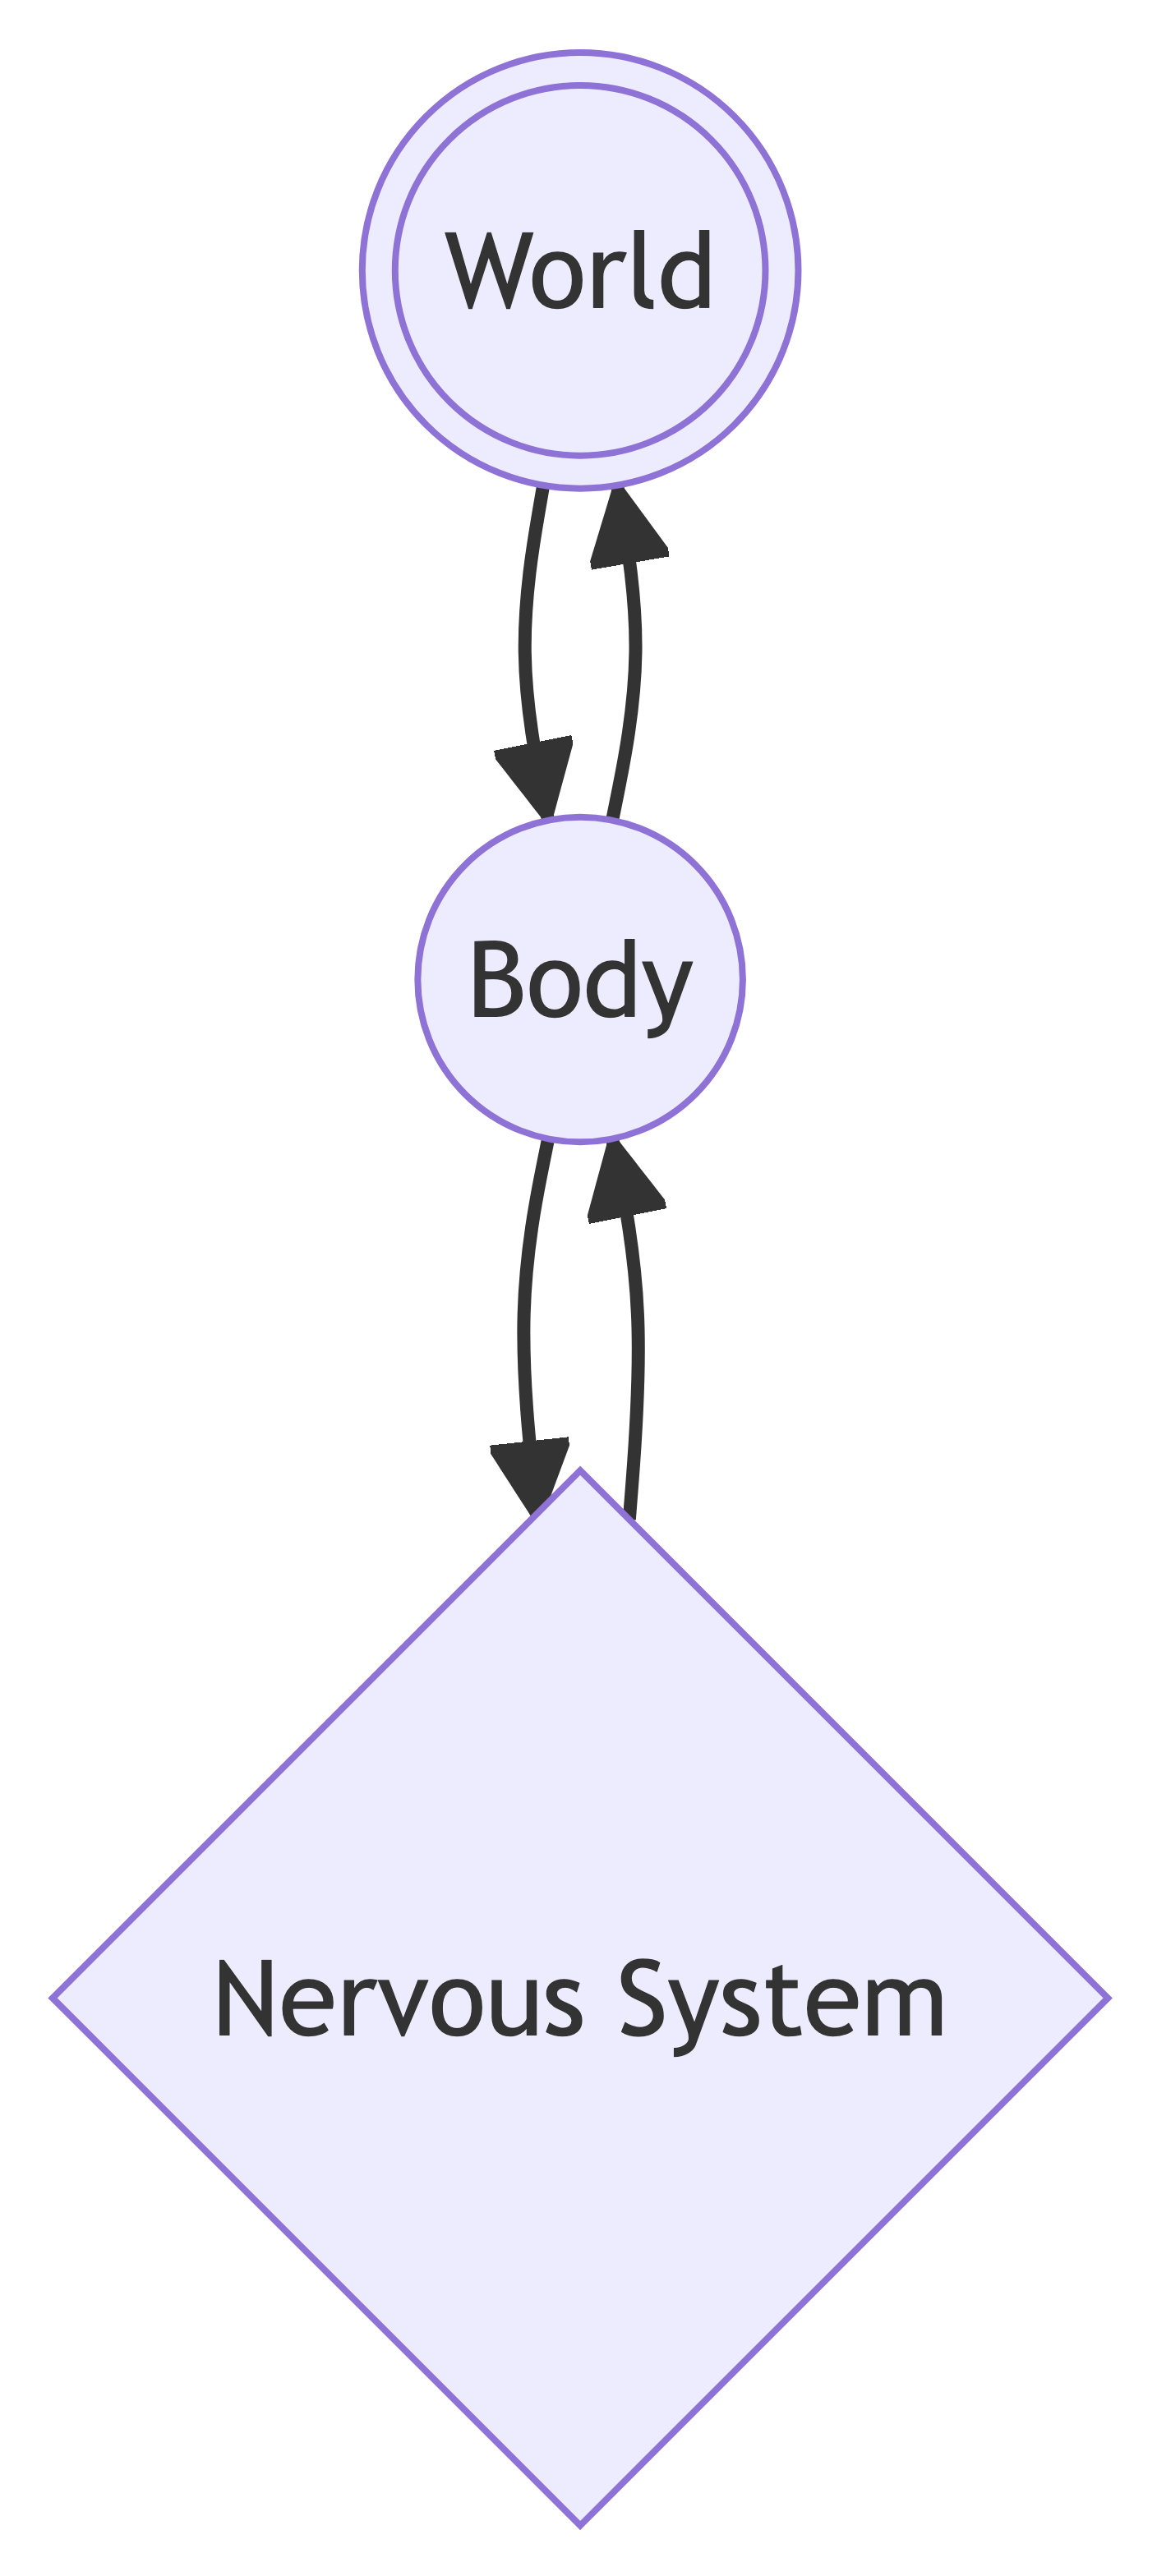
\includegraphics[width=1.84in,height=4.09in]{action_files/figure-latex/mermaid-figure-1.png}

A System of Systems

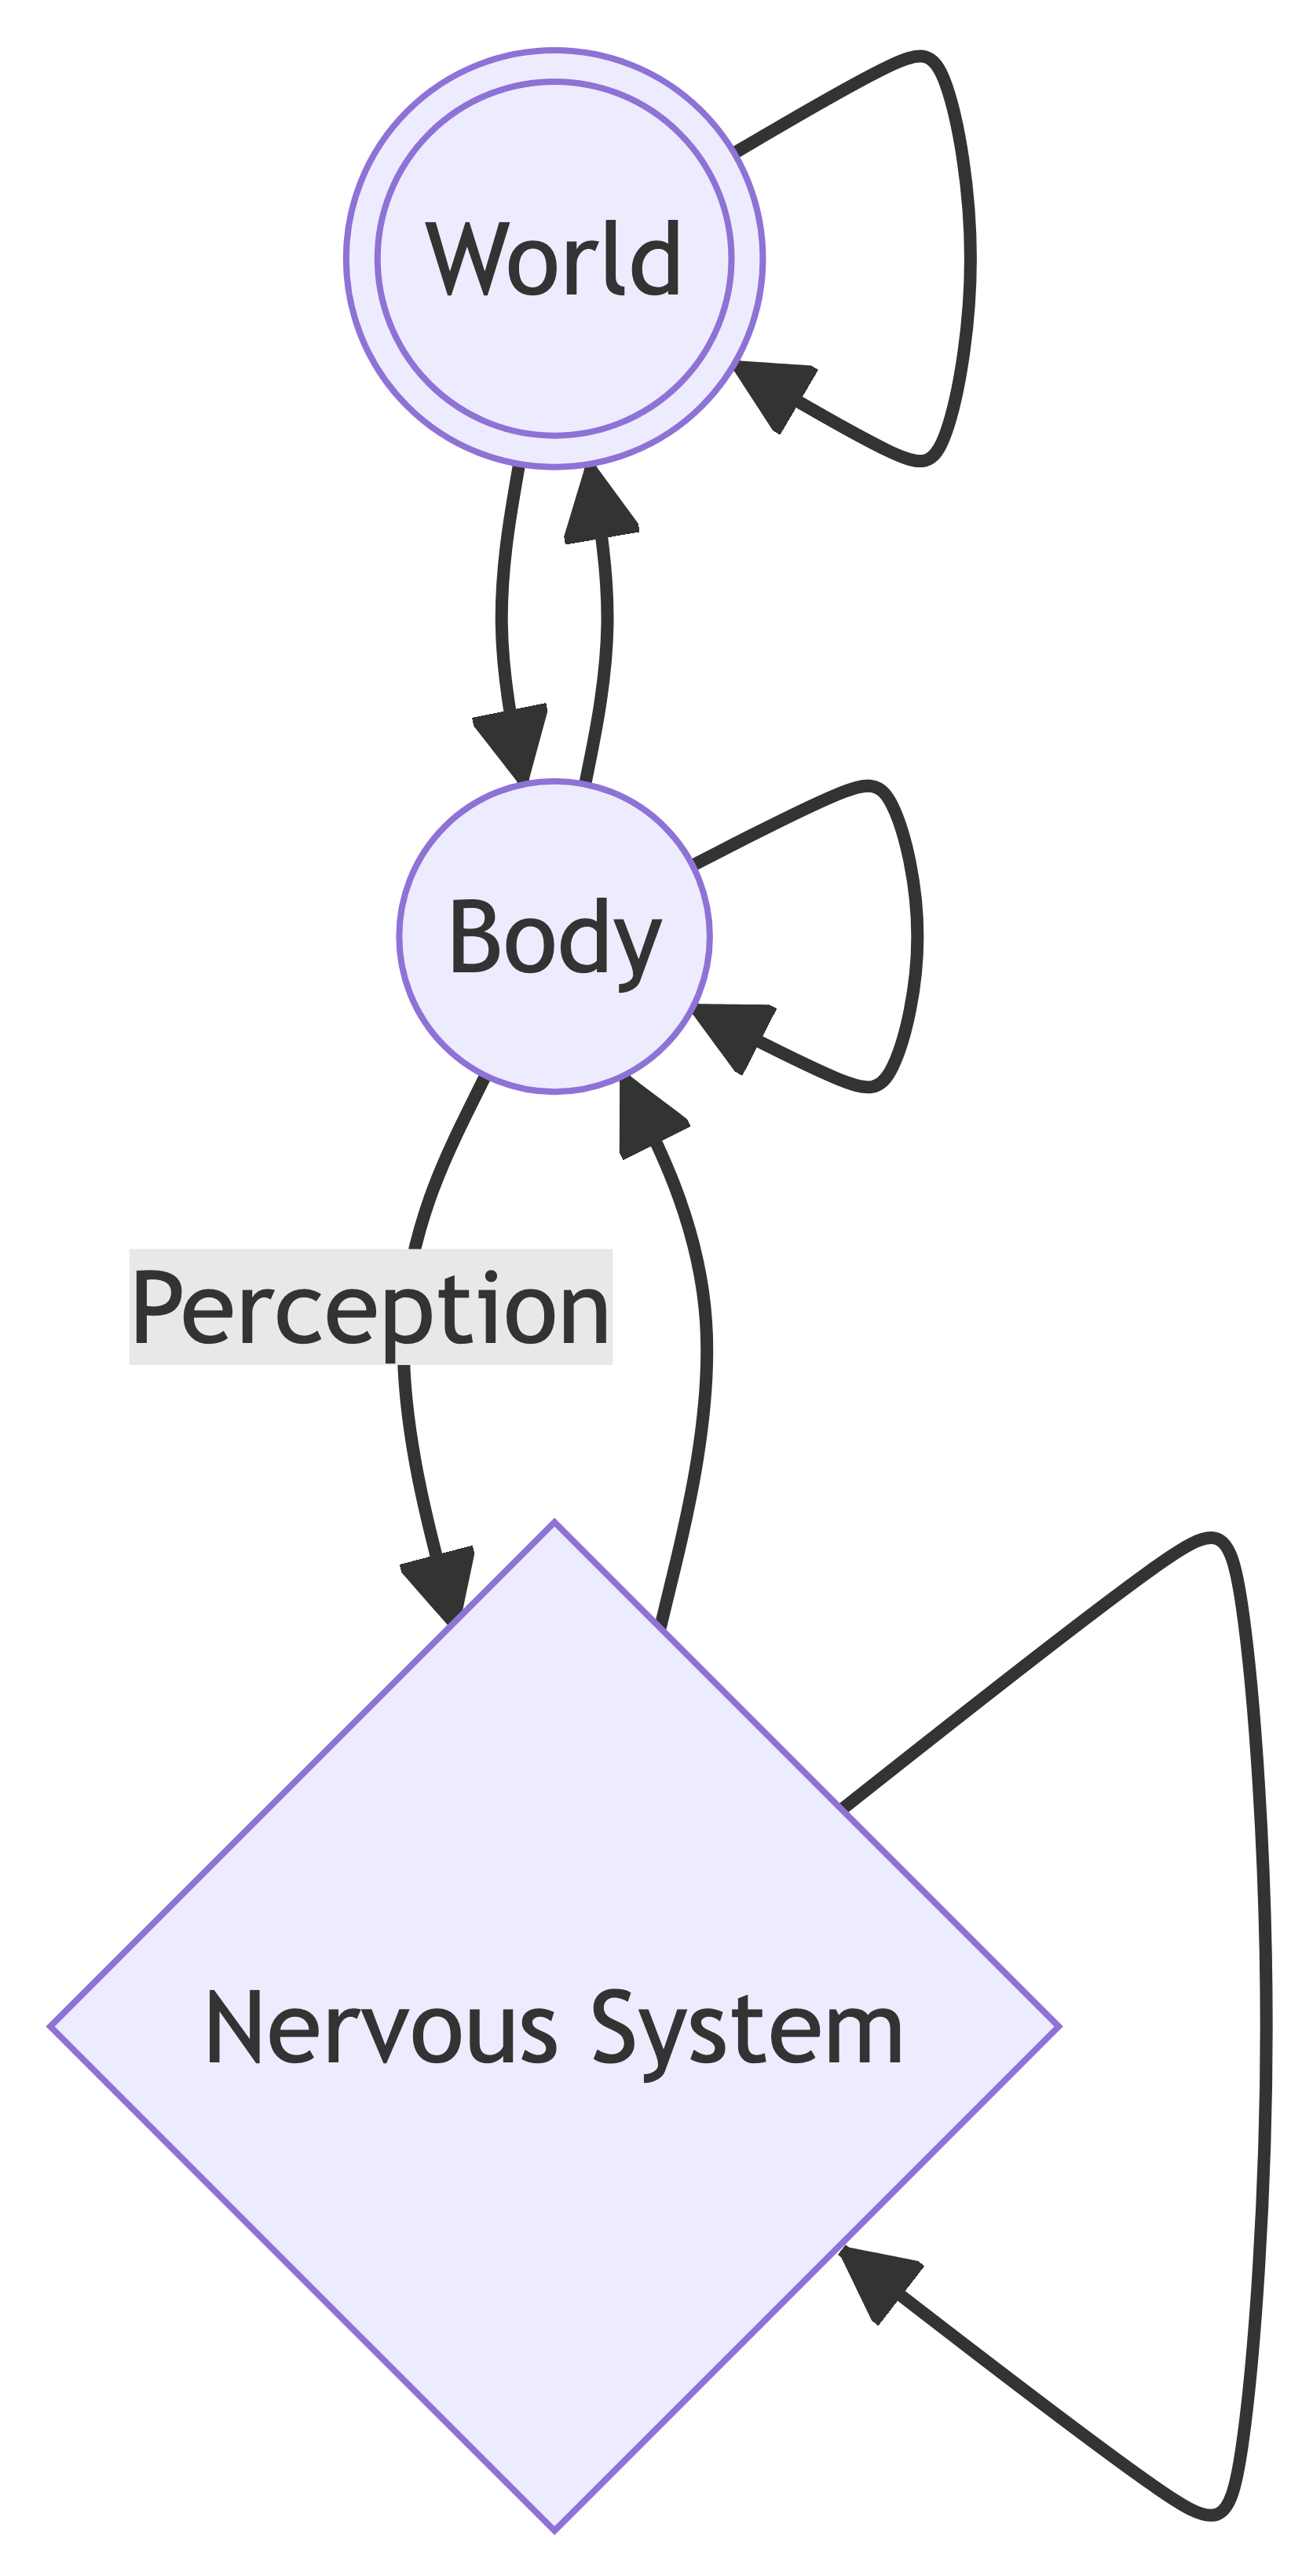
\includegraphics[width=2.18in,height=4.28in]{action_files/figure-latex/mermaid-figure-5.png}

With memory/momentum/inertia

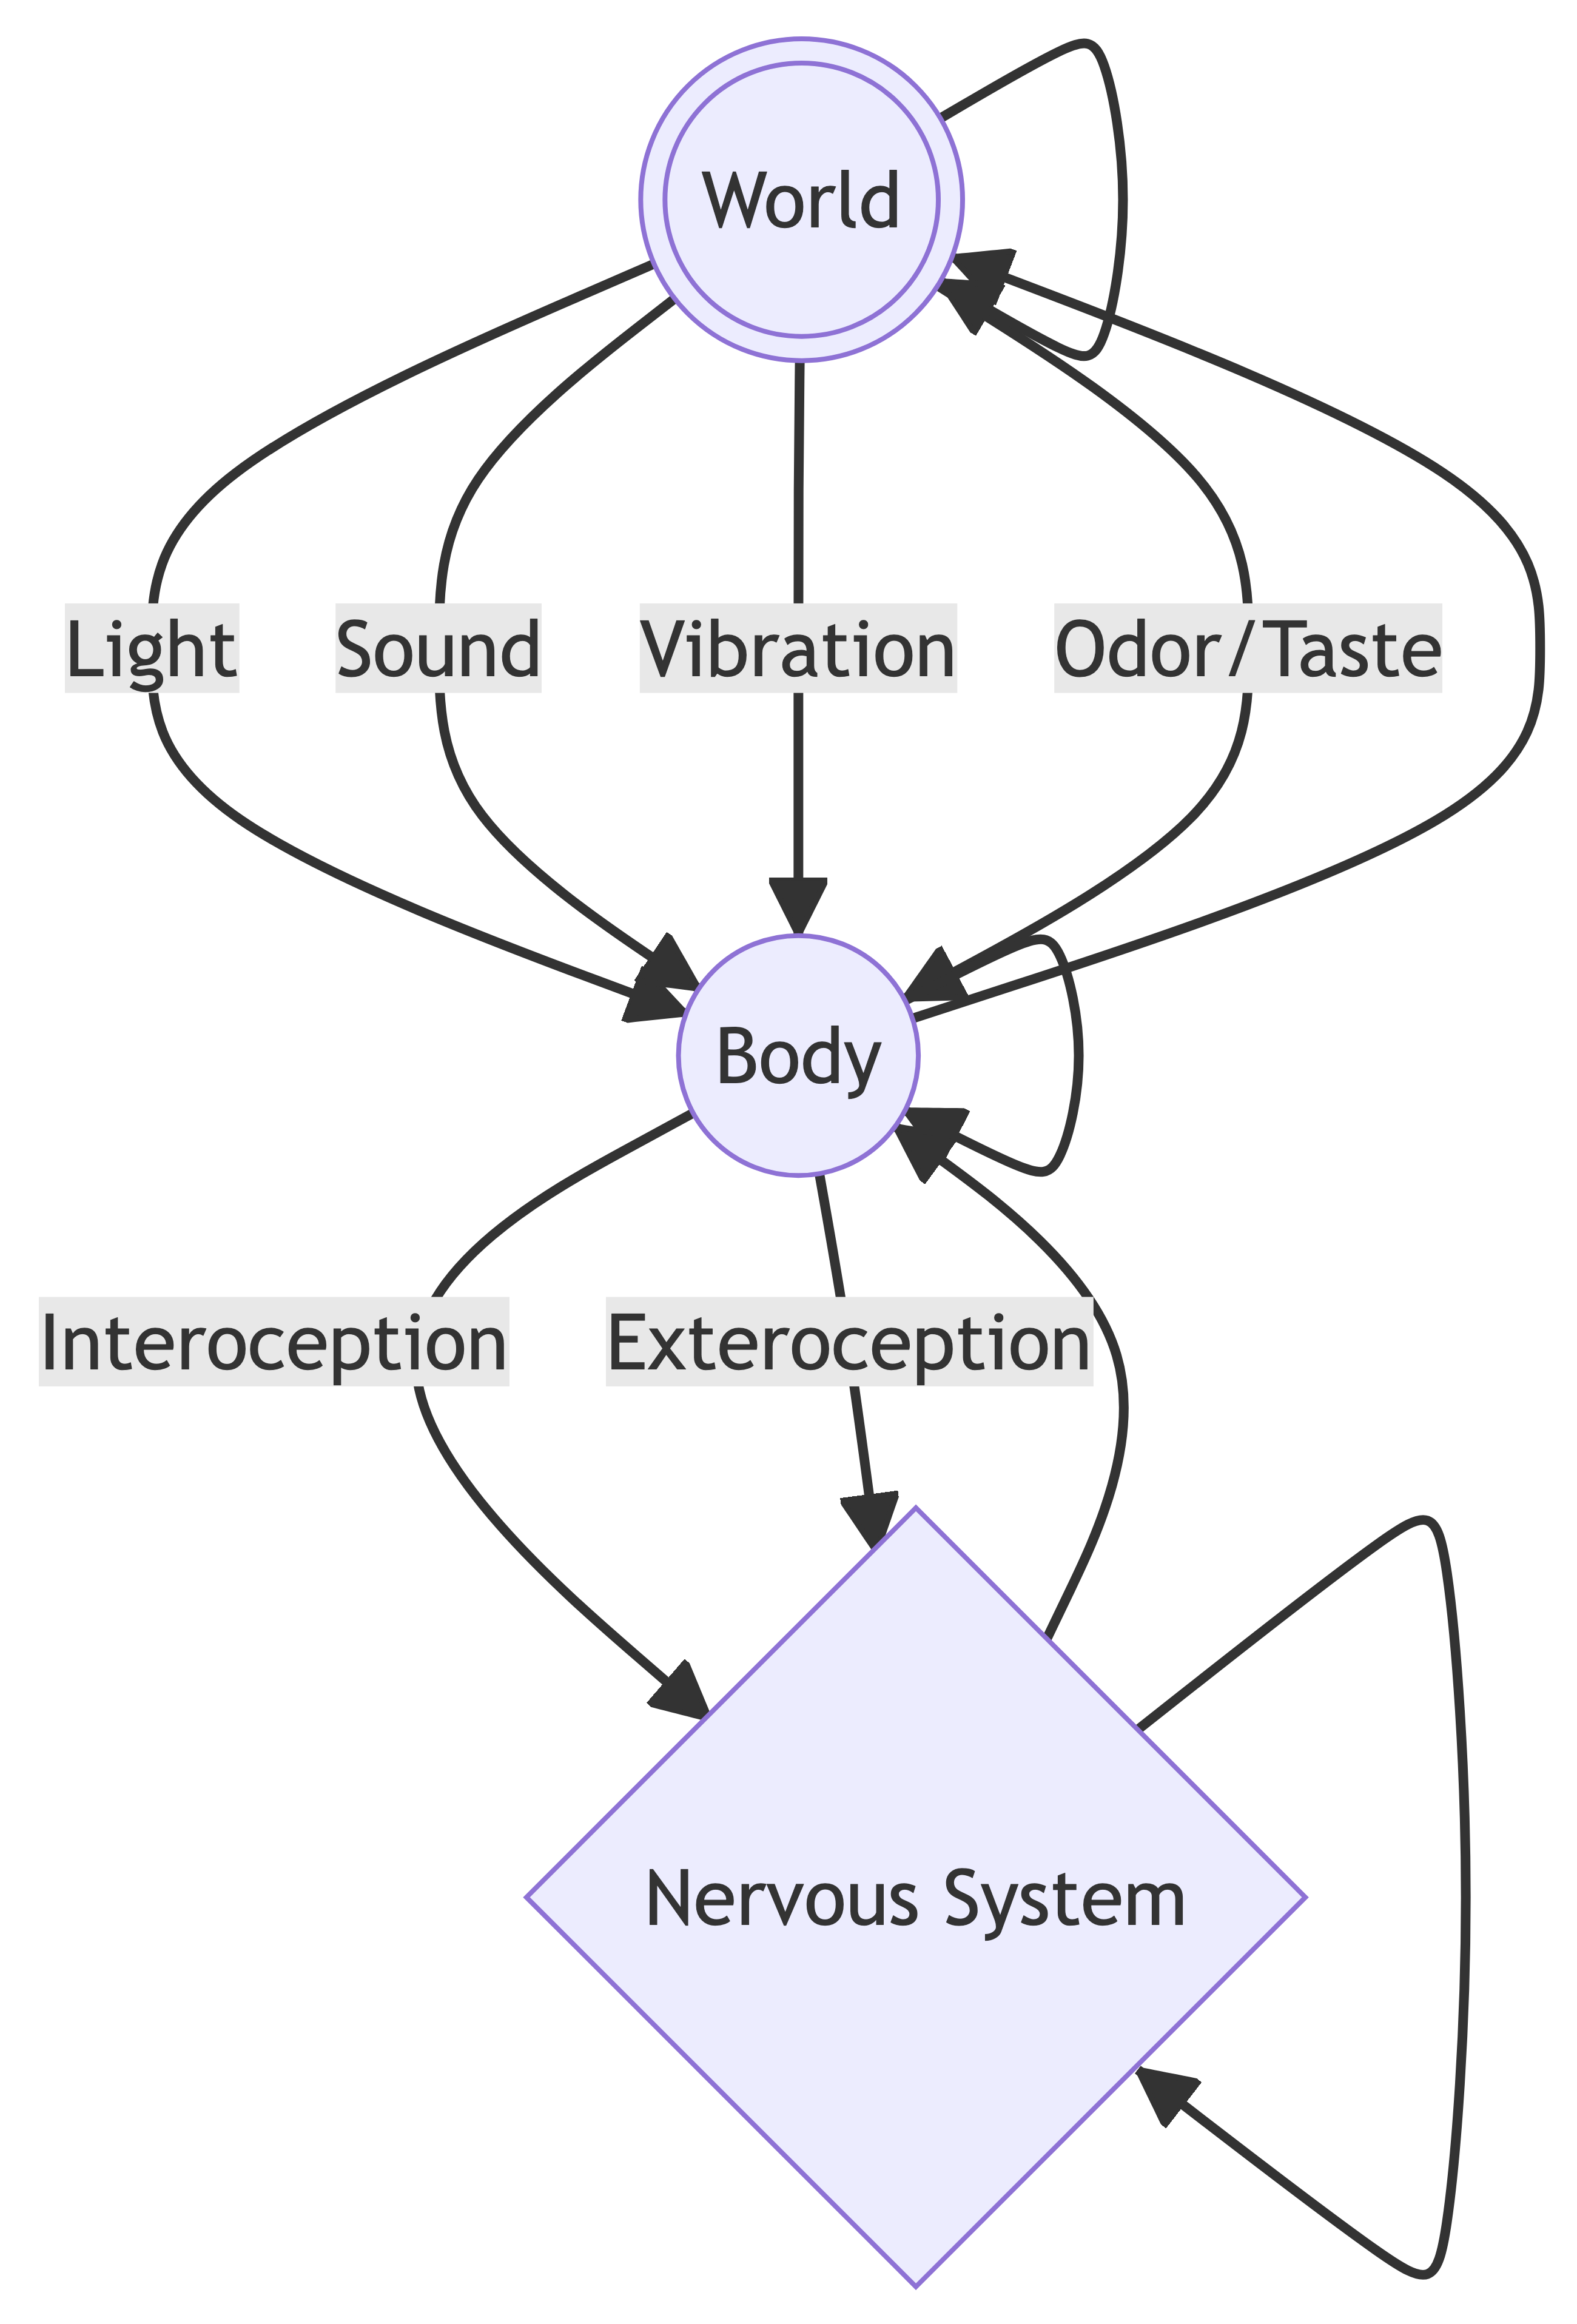
\includegraphics[width=3.39in,height=4.99in]{action_files/figure-latex/mermaid-figure-4.png}

Multiple input streams

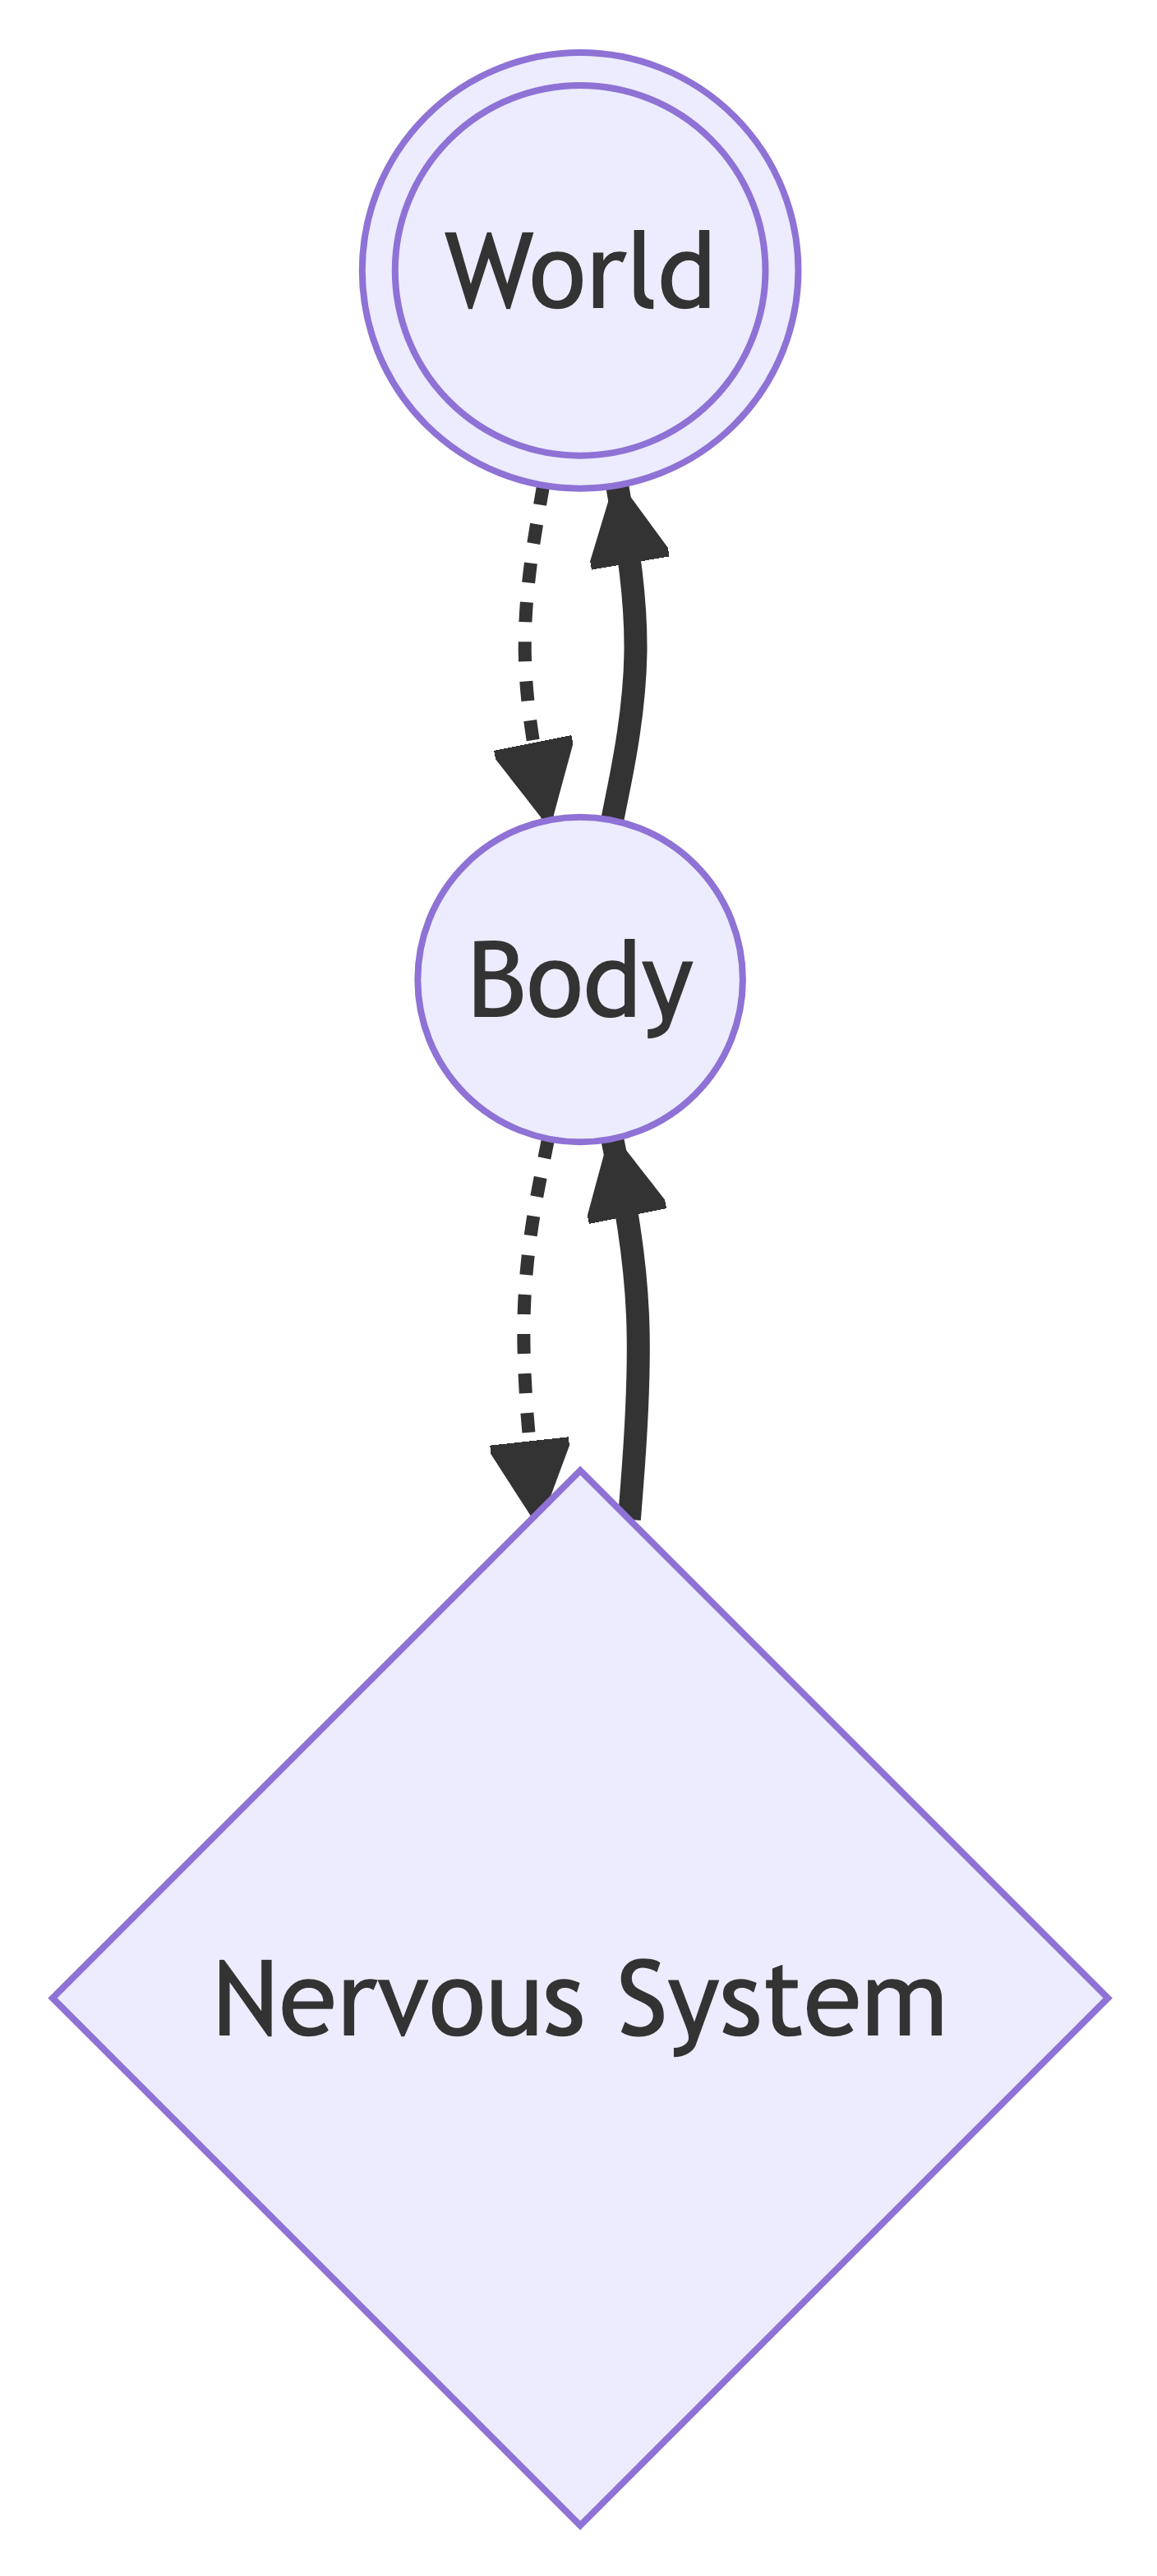
\includegraphics[width=1.84in,height=4.09in]{action_files/figure-latex/mermaid-figure-3.png}

Highlighting the output stream

\subsubsection{Our impact}\label{our-impact}

\begin{itemize}
\tightlist
\item
  What types of outputs are there?

  \begin{itemize}
  \tightlist
  \item
    Body to world?
  \item
    Nervous system to body?
  \end{itemize}
\item
  How are they produced?

  \begin{itemize}
  \tightlist
  \item
    By the muscles, glands
  \item
    By the nervous system
  \end{itemize}
\end{itemize}

\paragraph{\texorpdfstring{Body \(\rightarrow\)
World}{Body \textbackslash rightarrow World}}\label{body-rightarrow-world}

\begin{itemize}
\tightlist
\item
  Movements

  \begin{itemize}
  \tightlist
  \item
    Locomotion (move self)
  \item
    Manipulative (move other objects/entities)
  \item
    Communicative

    \begin{itemize}
    \tightlist
    \item
      Gestures
    \item
      Facial expressions
    \end{itemize}
  \end{itemize}
\item
  Secretions, excretions
\end{itemize}

\paragraph{\texorpdfstring{Nervous System \(\rightarrow\)
Body}{Nervous System \textbackslash rightarrow Body}}\label{nervous-system-rightarrow-body}

\begin{itemize}
\tightlist
\item
  Muscle commands
\item
  Autonomic responses
\item
  Endocrine responses
\end{itemize}

\paragraph{Physical considerations \&
constraints}\label{physical-considerations-constraints}

\begin{itemize}
\tightlist
\item
  \href{https://en.wikipedia.org/wiki/Animal_locomotion}{Medium/Environment}

  \begin{itemize}
  \tightlist
  \item
    Terrestrial
  \item
    Arborial
  \item
    Aerial
  \item
    Aquatic
  \item
    Fossorial
  \end{itemize}
\item
  External forces

  \begin{itemize}
  \tightlist
  \item
    Gravity
  \item
    Friction
  \item
    Drag
  \end{itemize}
\item
  Internal forces \& factors

  \begin{itemize}
  \tightlist
  \item
    Balance/orientation
  \item
    Reaction forces, complex dynamics
  \item
    Energetics
  \item
    Time delays
  \item
    Motor equivalence (Lashley, Bernstein)
  \end{itemize}
\end{itemize}

\begin{figure}[H]

{\centering 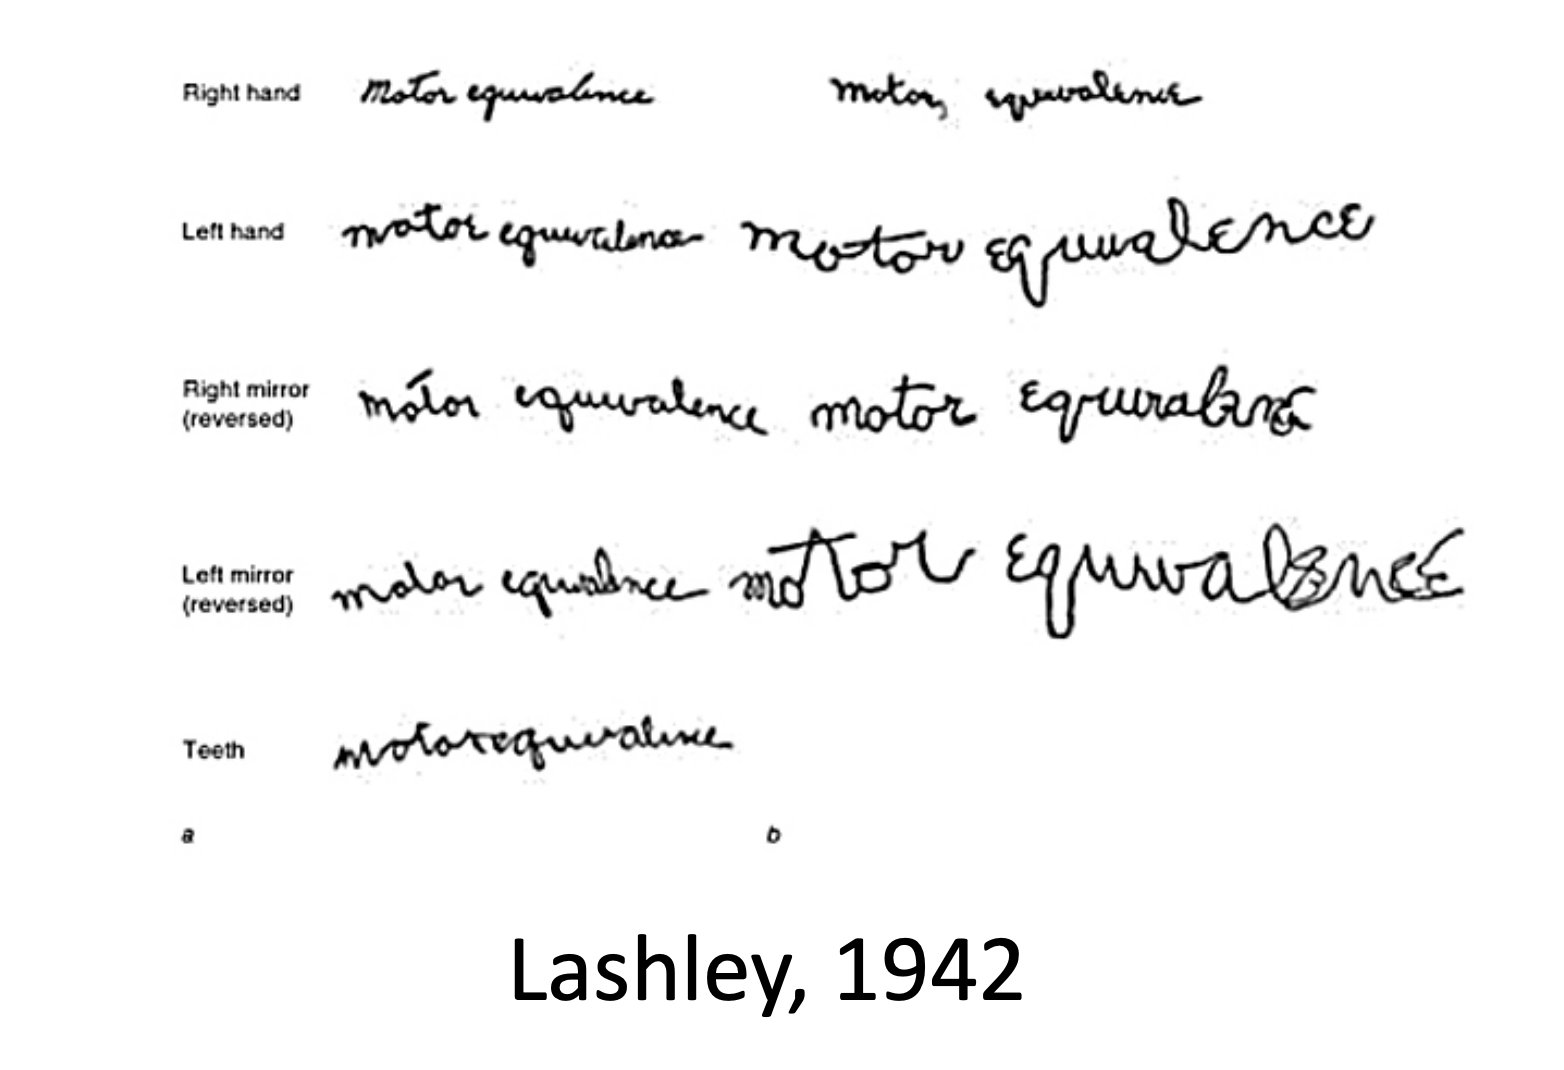
\includegraphics{../include/img/calliguri-motor-equivalance.png}

}

\caption{https://www.nist.gov/system/files/documents/oles/Michael-Caligiuri-NIST-2013-2.pdf}

\end{figure}%

\begin{itemize}
\tightlist
\item
  Frames of reference,
  \href{https://en.wikipedia.org/wiki/Degrees_of_freedom_problem\#}{degrees
  of freedom}
\end{itemize}

\begin{figure}[H]

{\centering \includegraphics{action_files/mediabag/lossless-page1-1136p.png}

}

\caption{Wikipedia. Cat hindlimb musculoskeletal model with redundant
degrees of freedom at muscles (red lines) and joints.}

\end{figure}%%
\begin{figure}[H]

{\centering 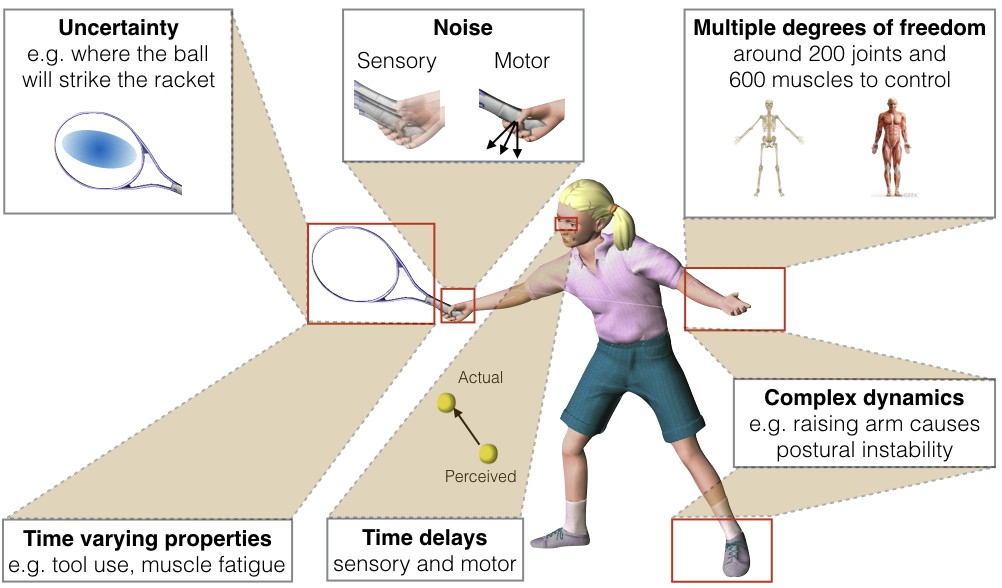
\includegraphics{action_files/mediabag/overview.jpg}

}

\caption{https://wolpertlab.neuroscience.columbia.edu/research-projects/overview.
Movement is the only way we have of interacting with the world, whether
foraging for food or attracting a waiter's attention. Therefore, the
purpose of the human brain is to use sensory signals to determine future
actions.}

\end{figure}%

\subsubsection{Psychological
considerations}\label{psychological-considerations}

\begin{itemize}
\tightlist
\item
  Foraging for

  \begin{itemize}
  \tightlist
  \item
    Food
  \item
    Shelter
  \item
    Mates
  \item
    Information
  \end{itemize}
\item
  Defending

  \begin{itemize}
  \tightlist
  \item
    Escaping predators
  \item
    Fighting
  \end{itemize}
\item
  Communicating
\item
  Playing
\end{itemize}

\subsubsection{Types of movements}\label{types-of-movements}

\begin{figure}[H]

{\centering 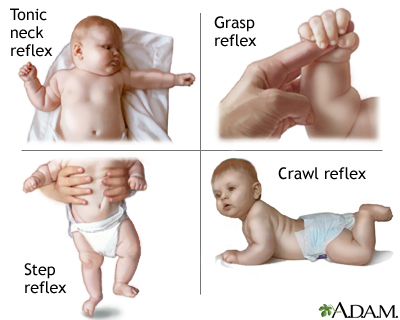
\includegraphics{action_files/mediabag/17234.jpg}

}

\caption{https://medlineplus.gov/ency/images/ency/fullsize/17234.jpg}

\end{figure}%

\begin{itemize}
\tightlist
\item
  Reflexes

  \begin{itemize}
  \tightlist
  \item
    Simple, highly stereotyped, unlearned, rapid, acquired early
  \end{itemize}
\end{itemize}

\begin{itemize}
\tightlist
\item
  vs.~planned or voluntary actions

  \begin{itemize}
  \tightlist
  \item
    Complex, flexible, acquired, slower
  \end{itemize}
\item
  Discrete (reaching) vs.~rhythmic (walking)
\item
  Ballistic (no feedback) vs.~controlled (feedback)
\end{itemize}

\subsection{Motor system anatomy}\label{motor-system-anatomy}

\subsubsection{Key `nodes'}\label{key-nodes}

\begin{figure}[H]

{\centering 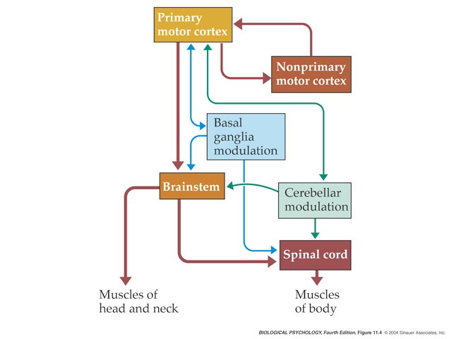
\includegraphics{../include/img/motor-controllers-biopsych.jpg}

}

\caption{\emph{Biological Psychology 4th ed}}

\end{figure}%

\begin{itemize}
\tightlist
\item
  Primary motor cortex (M1)
\end{itemize}

\begin{figure}[H]

{\centering \includegraphics{action_files/mediabag/Blausen_0103_Brain_S.png}

}

\caption{M1. Wikipedia:
\url{https://en.wikipedia.org/wiki/Primary_motor_cortex}}

\end{figure}%%
\begin{figure}[H]

{\centering \includegraphics{action_files/mediabag/1920px-Motor_homuncu.png}

}

\caption{Motor homunculus. Wikipedia}

\end{figure}%

\begin{itemize}
\tightlist
\item
  Non-primary motor cortex
\item
  Basal ganglia
\item
  Brain stem
\item
  Cerebellum
\item
  Spinal cord
\end{itemize}

\subsubsection{Projection pathways}\label{projection-pathways}

\paragraph{Pyramidal tracts}\label{pyramidal-tracts}

\begin{itemize}
\tightlist
\item
  Pyramidal cells

  \begin{itemize}
  \tightlist
  \item
    Cerebral Cortex Layer 5 in primary motor cortex (M1)
  \end{itemize}
\item
  Corticobulbar (cortex -\textgreater{} brainstem) tract
\item
  Corticospinal (cortex -\textgreater{} spinal cord) tract
\item
  Crossover (decussate) in medulla

  \begin{itemize}
  \tightlist
  \item
    L side of brain ennervates R side of body
  \end{itemize}
\end{itemize}

\begin{figure}[H]

{\centering 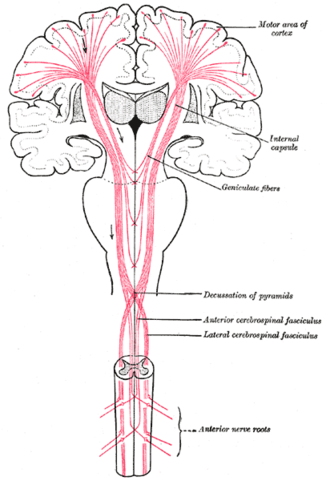
\includegraphics{../include/img/gray-corticospinal-tract.png}

}

\caption{Source: Wikipedia}

\end{figure}%

\begin{tcolorbox}[enhanced jigsaw, leftrule=.75mm, opacityback=0, colbacktitle=quarto-callout-note-color!10!white, rightrule=.15mm, arc=.35mm, coltitle=black, breakable, colframe=quarto-callout-note-color-frame, toprule=.15mm, bottomrule=.15mm, opacitybacktitle=0.6, bottomtitle=1mm, titlerule=0mm, toptitle=1mm, colback=white, left=2mm, title=\textcolor{quarto-callout-note-color}{\faInfo}\hspace{0.5em}{Note}]

\begin{itemize}
\tightlist
\item
  Anatomically separate ascending (afferent) and descending (efferent)
  pathways in the spinal cord.
\item
  Ascending (generally) more dorsal; descending more ventral.
\item
  White matter on exterior (unlike cerebral cortex).
\end{itemize}

\end{tcolorbox}

\begin{figure}[H]

{\centering \includegraphics{action_files/mediabag/Gray672.png}

}

\caption{Source: Wikipedia}

\end{figure}%

\paragraph{Extrapyramidal system}\label{extrapyramidal-system}

\begin{itemize}
\tightlist
\item
  \href{https://en.wikipedia.org/wiki/Tectospinal_tract}{Tectospinal
  tract}
\item
  \href{https://en.wikipedia.org/wiki/Lateral_vestibulospinal_tract}{Lateral
  Vestibulospinal tract}
\item
  \href{https://en.wikipedia.org/wiki/Reticular_formation\#Descending_reticulospinal_tracts}{Reticulospinal
  tract}
\item
  Rubrospinal tract
\item
  \href{https://en.wikipedia.org/wiki/Extrapyramidal_symptoms}{Involuntary
  movements}

  \begin{itemize}
  \tightlist
  \item
    Posture, balance, arousal
  \end{itemize}
\end{itemize}

\subsubsection{Direct cortical control}\label{direct-cortical-control}

\begin{itemize}
\tightlist
\item
  Over \emph{some} motor neurons.
\item
  In humans; prevalence uncertain in other animals
\item
  For individuated (``fractionated'') movements of fingers, toes, lips,
  but other muscles, too.
\end{itemize}

\begin{figure}[H]

{\centering \includegraphics{action_files/mediabag/ne390081.f1.gif}

}

\caption{{[}@Nielsen2016-hs{]}. Figure 1. Evidence of
corticomotoneuronal connections in human subjects. Indirect, noninvasive
evidence of the existence of monosynaptic connections between
corticospinal neurons and spinal motoneurons may be obtained in awake
human subjects by transcranial magnetic stimulation (TMS) (b,c) and
coherence analysis of either cortical {[}electroencephalogram (EEG){]}
and muscular activity {[}electromyogram (EMG){]} (d,e) or two separate
recordings of muscular activity (f). (b,c) Corticospinal neurons can be
excited by a brief magnetic pulse applied by a magnetic coil placed over
the appropriate part of the motor cortex in awake human subjects. If the
intensity of the magnetic pulse is adjusted appropriately, the evoked
descending volley in the corticospinal tract may elicit a subthreshold
excitatory postsynaptic potential (EPSP) in the relevant spinal
motoneurons. This EPSP may be demonstrated as a change in the discharge
probability of a single motor unit recorded from the muscle (b). In the
illustrated example, the subject was asked to voluntarily activate the
tibialis anterior (TA) muscle, and the discharges of a single motor unit
were recorded by a needle electrode inserted into the muscle. TMS
elicited a short-lasting (2-ms) increase of discharge probability at a
latency of 45 ms (b). The short duration of this peak is consistent with
the short rise time of a monosynaptic EPSP. This interpretation is
further supported by the observation that stimulation of Ia afferents
with known monosynaptic connections to the motoneurons elicits a peak
with a similar short duration (c). Data in panels b and c modified with
permission from Nielsen \& Petersen (1994). (d,e) EEG recorded from the
motor cortex and EMG recorded from a voluntarily activated muscle (TA in
the illustrated example) show rhythmic modulation of the recorded
activity at a frequency of 15--35 Hz. As shown from a coherence analysis
of the two signals in panel d, some of this activity is common for the
two sites, suggesting a close link between cortical and muscular
activity. Panel e shows the EEG and EMG activities are not always
synchronous but may show a time lag, which is in the range expected for
a fast-conducting direct pathway to the motoneurons. Data in panels d
and e modified with permission from Hansen et al.~(2002). (f) A
monosynaptic origin of corticomuscular coherence is further supported by
the observation of short-term synchrony between the discharges of pairs
of TA motor units, which may be related to the coherence in the
15--35-Hz frequency band. The subject was asked to voluntarily activate
the TA muscle, and the discharges of two different TA motor units were
recorded with needle electrodes. The short duration of the central peak
of synchronization suggests that the motor unit activities are modulated
by a common (monosynaptic) input from collaterals of last-order neurons,
which are in all likelihood identical to corticomotoneuronal cells. The
secondary peaks at lags of approximately 50--60 ms on either side of the
central peak suggest that this last-order input modulates the discharge
of the motor units at a frequency of about 20--30 Hz, i.e.,
corresponding to the coherence observed in the paired EEG-EMG recordings
in panels b and c.~Data in panel f modified with permission from Nielsen
\& Kagamihara (1994).}

\end{figure}%

\subsection{Muscles}\label{muscles}

\begin{itemize}
\tightlist
\item
  Generate forces
\item
  In one direction
\end{itemize}

\subsubsection{Functional classes}\label{functional-classes}

\begin{itemize}
\tightlist
\item
  Axial

  \begin{itemize}
  \tightlist
  \item
    Trunk, neck, hips
  \end{itemize}
\item
  Proximal

  \begin{itemize}
  \tightlist
  \item
    Shoulder/elbow, pelvis/knee
  \end{itemize}
\item
  Distal

  \begin{itemize}
  \tightlist
  \item
    Hands/fingers, feet/toes
  \end{itemize}
\end{itemize}

\begin{figure}[H]

{\centering 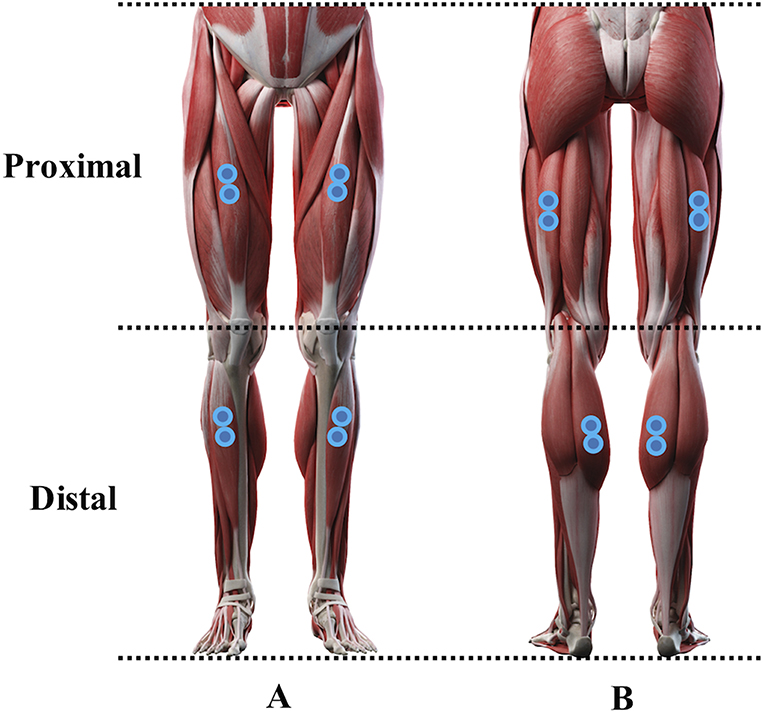
\includegraphics{action_files/mediabag/fneur-10-00951-g001.jpg}

}

\caption{{[}@Cantu2019-sz{]}}

\end{figure}%

\subsubsection{Agonist/antagonist pairs}\label{agonistantagonist-pairs}

\begin{center}
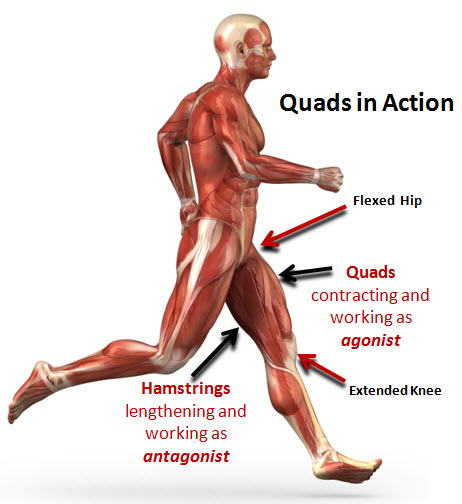
\includegraphics{action_files/mediabag/Hamstring-Quad4.jpg}
\end{center}

\subsubsection{Anatomical types}\label{anatomical-types}

\begin{center}
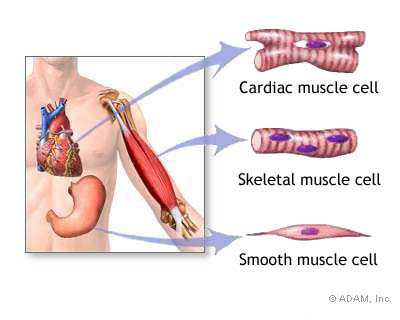
\includegraphics{action_files/mediabag/19917.jpg}
\end{center}

\begin{itemize}
\tightlist
\item
  Cardiac
\item
  Striated (striped)

  \begin{itemize}
  \tightlist
  \item
    Skeletal muscles
  \item
    Voluntary control, mostly connected to tendons and bones
  \end{itemize}
\item
  Smooth

  \begin{itemize}
  \tightlist
  \item
    Arteries, hair follicles, uterus, intestines
  \item
    Regulated by ANS (involuntary)
  \end{itemize}
\end{itemize}

\subsubsection{How skeletal muscles
contract}\label{how-skeletal-muscles-contract}

\begin{itemize}
\tightlist
\item
  Motor neurons (cell bodies located in ventral horn of spinal cord)
\item
  Project to muscle fiber
\item
  Form neuromuscular junction

  \begin{itemize}
  \tightlist
  \item
    Synapse between motor neuron and muscle fiber
  \item
    Release acetylcholine (ACh)
  \end{itemize}
\end{itemize}

\begin{figure}[H]

{\centering 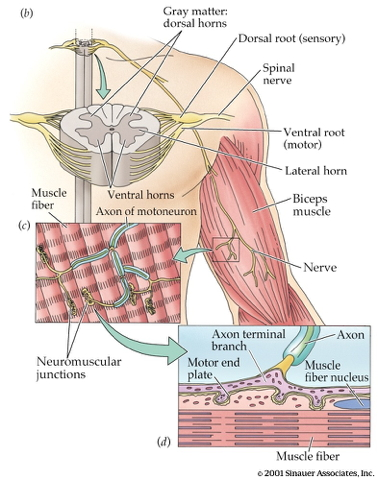
\includegraphics{../include/img/from-spinal-cord-to-muscle.jpg}

}

\caption{\emph{Biological Psychology 4th ed.}}

\end{figure}%

\begin{itemize}
\tightlist
\item
  Motor endplate

  \begin{itemize}
  \tightlist
  \item
    Contains nicotinic ACh receptors
  \end{itemize}
\item
  Activation produces excitatory endplate potential

  \begin{itemize}
  \tightlist
  \item
    Muscle fibers depolarize
  \item
    Depolarization spreads along fibers like an action potential
  \item
    Ca++ released from intramuscular stores
  \end{itemize}
\end{itemize}

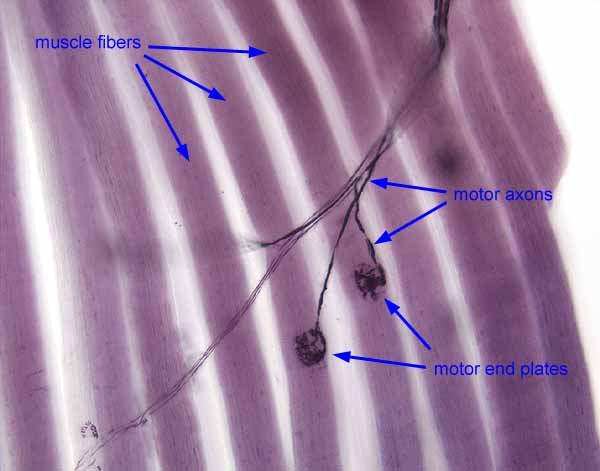
\includegraphics{action_files/mediabag/NM040b.jpg}

\begin{itemize}
\tightlist
\item
  Myofibrils

  \begin{itemize}
  \tightlist
  \item
    Contain actin \& mysosin proteins
  \item
    ``Molecular gears''
  \end{itemize}
\item
  Muscle fibers contain bundles of myofibrils called sarcomeres

  \begin{itemize}
  \tightlist
  \item
    Bind, move, unbind in presence of Ca++, adenosine triphosphate (ATP)
  \end{itemize}
\end{itemize}

\begin{center}
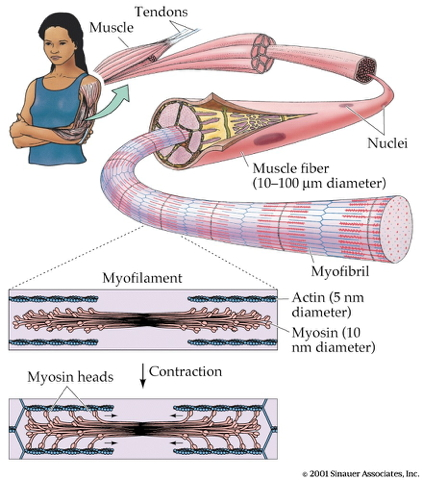
\includegraphics{../include/img/muscle-fibers-biopsych.jpg}
\end{center}

\begin{center}
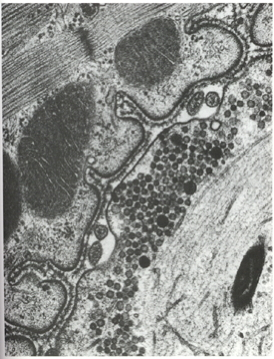
\includegraphics{../include/img/motor-endplate-nt-release.jpg}
\end{center}

\subsubsection{Skeletal muscle fiber
types}\label{skeletal-muscle-fiber-types}

\begin{center}
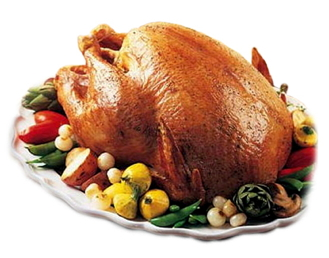
\includegraphics{../include/img/turkey.jpg}
\end{center}

\begin{itemize}
\tightlist
\item
  Fast twitch/fatiguing

  \begin{itemize}
  \tightlist
  \item
    Type II
  \item
    White meat
  \end{itemize}
\item
  Slow twitch/fatiguing

  \begin{itemize}
  \tightlist
  \item
    Type I
  \item
    Red meat
  \end{itemize}
\end{itemize}

\subsubsection{Muscles as sensory
organs}\label{muscles-as-sensory-organs}

\begin{center}

\includegraphics{action_files/mediabag/canstock6466988.jpg}
\end{center}

\paragraph{Two skeletal muscle fiber
types}\label{two-skeletal-muscle-fiber-types}

\begin{center}
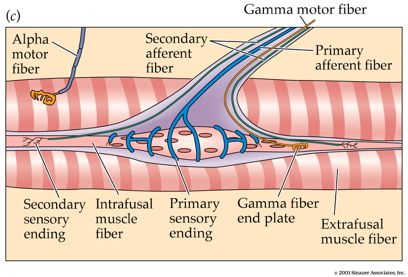
\includegraphics{../include/img/muscle-fiber-types.jpg}
\end{center}

\subparagraph{Intrafusal fibers}\label{intrafusal-fibers}

\begin{itemize}
\tightlist
\item
  Sense muscle length and change in length, e.g.~``stretch''
\item
  Also called muscle spindles
\item
  Provide muscle proprioception (perception about the self, a form of
  interoception)
\item
  Sensory function

  \begin{itemize}
  \tightlist
  \item
    Ennervated by by primary Ia afferents (sensory output from muscle)
  \item
    Secondary Type II fibers
  \end{itemize}
\item
  Motor function

  \begin{itemize}
  \tightlist
  \item
    Ennervated by gamma (\(\gamma\)) motor neurons (motor input)
  \end{itemize}
\end{itemize}

\subparagraph{Extrafusal fibers}\label{extrafusal-fibers}

\begin{itemize}
\tightlist
\item
  Generate force
\item
  ennervated by alpha (\(\alpha\)) motor neurons
\item
  No ``sensory'' role, except for \emph{efference copy}

  \begin{itemize}
  \tightlist
  \item
    ``Copies'' of motor output sent to other brain areas
  \end{itemize}
\end{itemize}

\subsubsection{Monosynaptic stretch (myotatic)
reflex}\label{monosynaptic-stretch-myotatic-reflex}

\begin{itemize}
\tightlist
\item
  Muscle stretched (length increases)
\item
  Muscle spindle in intrafusal fiber activates
\item
  Ia afferent sends signal to spinal cord

  \begin{itemize}
  \tightlist
  \item
    Activates alpha (\(\alpha\)) motor neuron
  \end{itemize}
\item
  Muscle contracts, shortens length
\end{itemize}

\begin{figure}[H]

{\centering \includegraphics{action_files/mediabag/Fusimotor_action.jpg}

}

\caption{Source: Wikipedia}

\end{figure}%

\begin{itemize}
\tightlist
\item
  Gamma (\(\gamma\)) motor neuron fires to take up `slack' in intrafusal
  fiber
\end{itemize}

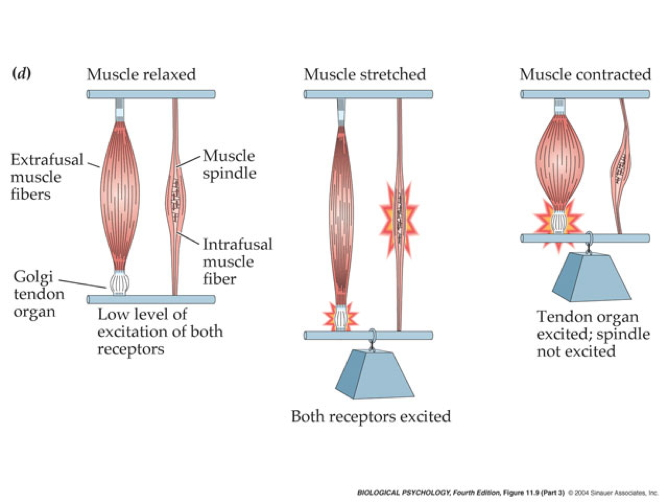
\includegraphics{../include/img/intrafusal-extrafusal-fibers.jpg}

\begin{tcolorbox}[enhanced jigsaw, leftrule=.75mm, opacityback=0, colbacktitle=quarto-callout-note-color!10!white, rightrule=.15mm, arc=.35mm, coltitle=black, breakable, colframe=quarto-callout-note-color-frame, toprule=.15mm, bottomrule=.15mm, opacitybacktitle=0.6, bottomtitle=1mm, titlerule=0mm, toptitle=1mm, colback=white, left=2mm, title=\textcolor{quarto-callout-note-color}{\faInfo}\hspace{0.5em}{Note}]

This is a bit like the role of a belayer in rock climbing.

\includegraphics{action_files/mediabag/HowtoBelay_3-5711179.webp}

\end{tcolorbox}

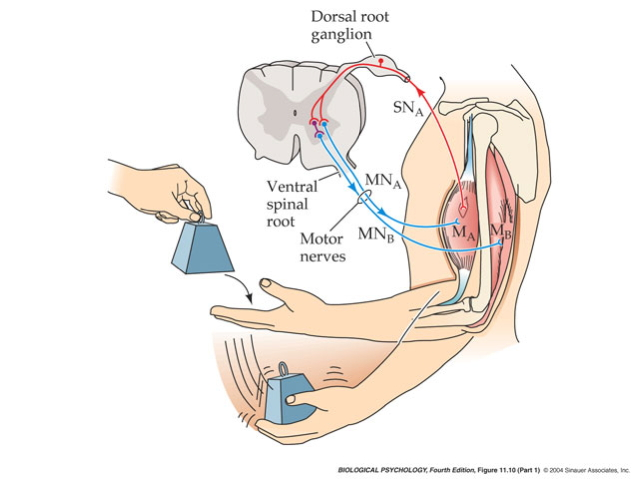
\includegraphics{../include/img/stretch-reflex.jpg}

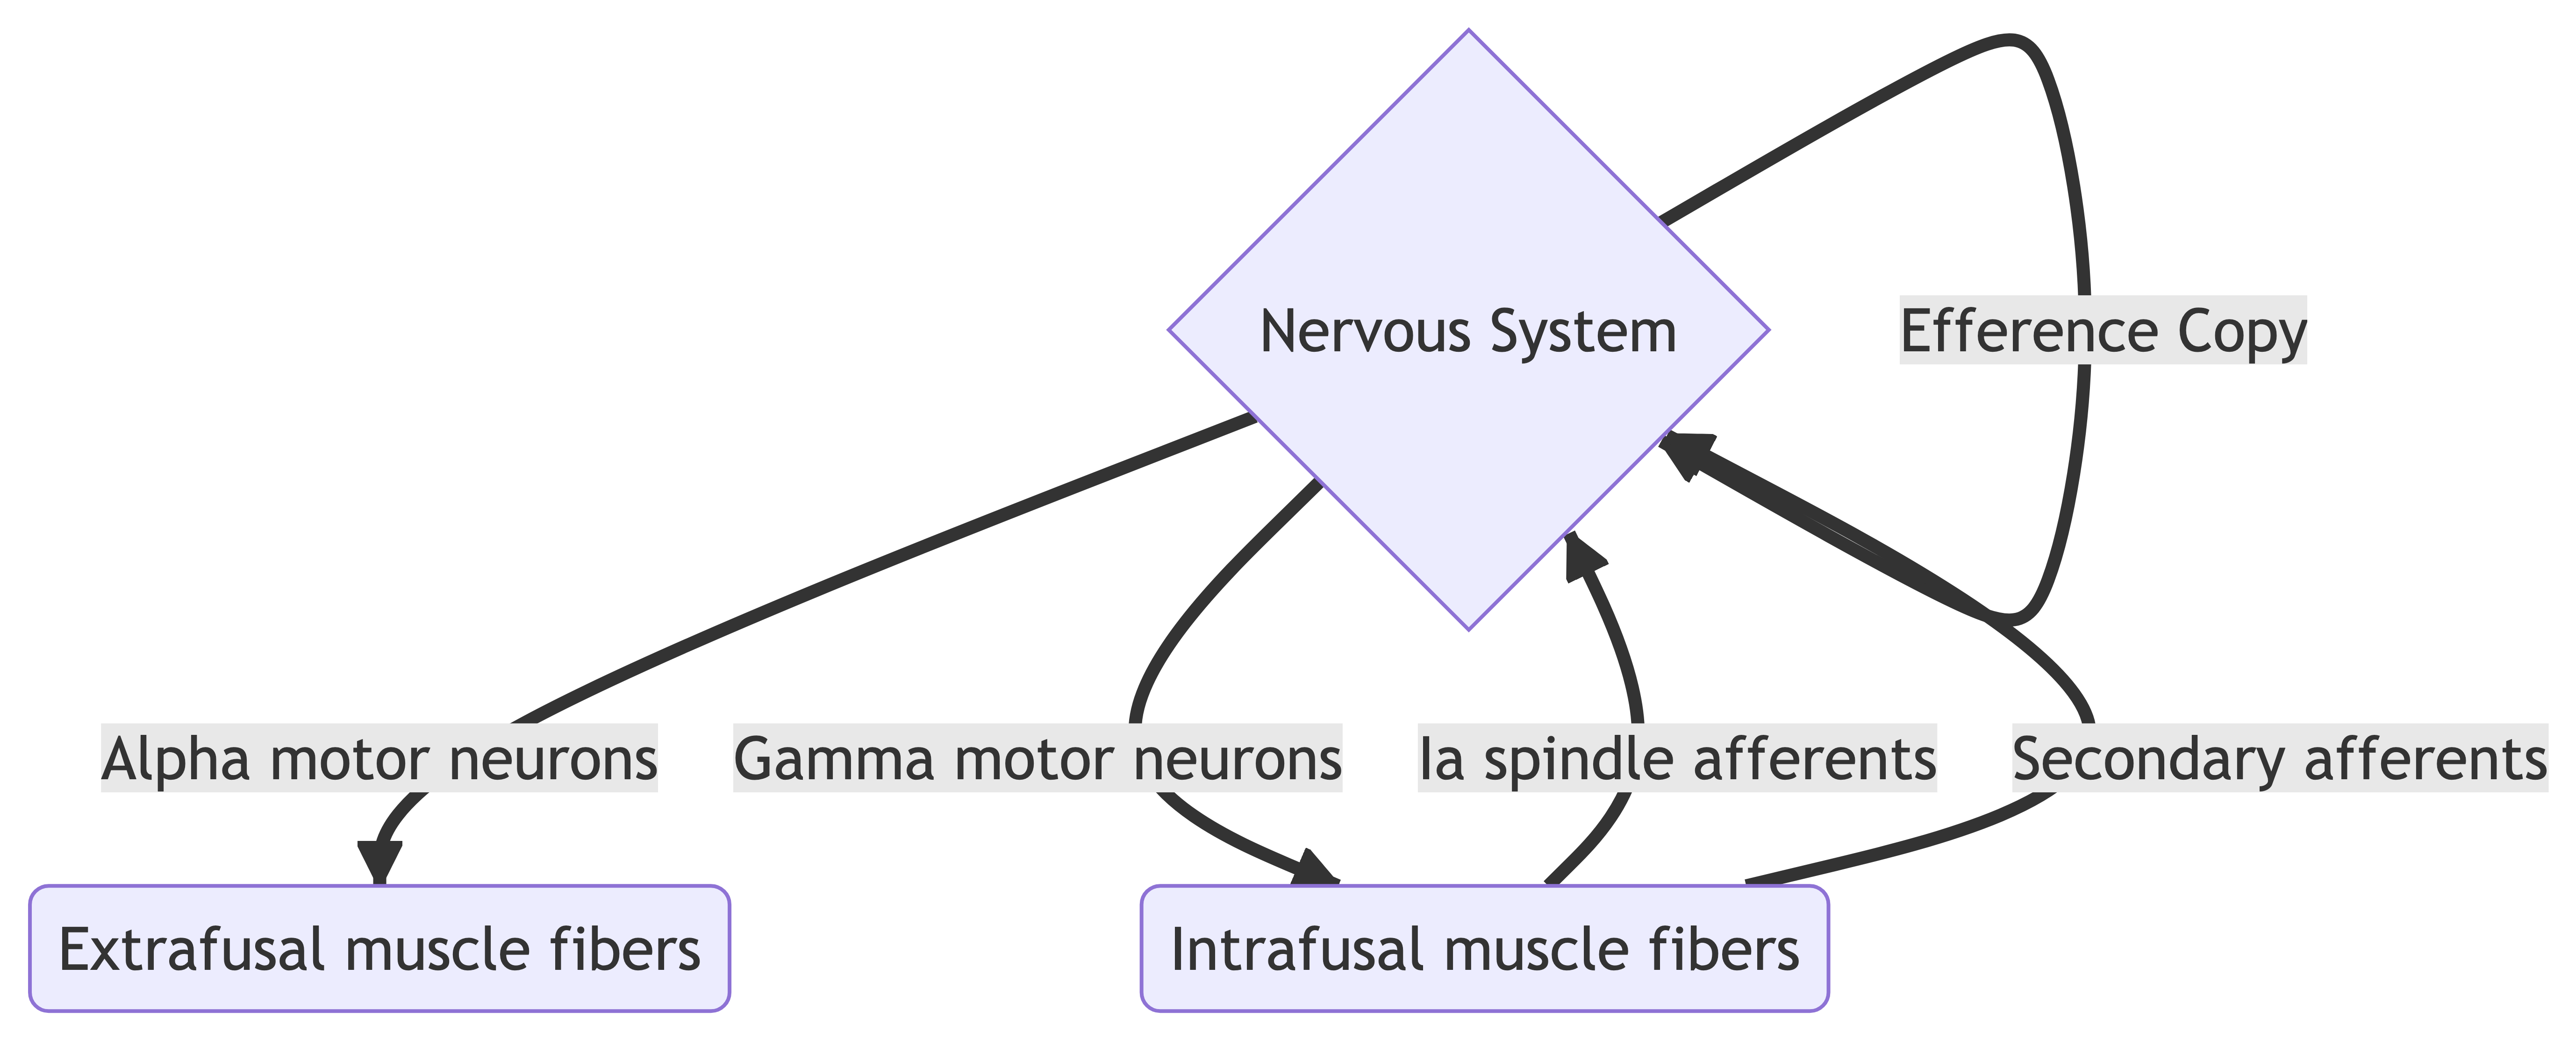
\includegraphics[width=7.18in,height=2.9in]{action_files/figure-latex/mermaid-figure-2.png}

Highlighting the output stream

\paragraph{Why doesn't antagonist muscle
respond?}\label{why-doesnt-antagonist-muscle-respond}

\begin{itemize}
\tightlist
\item
  Polysynaptic inhibition of antagonist muscle
\item
  Prevents/dampens tremor
\end{itemize}

\begin{tcolorbox}[enhanced jigsaw, leftrule=.75mm, opacityback=0, colbacktitle=quarto-callout-note-color!10!white, rightrule=.15mm, arc=.35mm, coltitle=black, breakable, colframe=quarto-callout-note-color-frame, toprule=.15mm, bottomrule=.15mm, opacitybacktitle=0.6, bottomtitle=1mm, titlerule=0mm, toptitle=1mm, colback=white, left=2mm, title=\textcolor{quarto-callout-note-color}{\faInfo}\hspace{0.5em}{Note}]

How does the motor system ``learn'' the sensory consequences of muscle
fiber contraction? Could spontaneous ``twitches'' be involved
{[}@Blumberg2023-ce{]}?

That is, higher levels of the nervous system learn the relationship
between motor neuron output and spindle feedback.

\end{tcolorbox}

\paragraph{Speed of sensory information
propagation}\label{speed-of-sensory-information-propagation}

\begin{itemize}
\tightlist
\item
  Brain gets fast(est) propagating sensory info from muscle spindles
\end{itemize}

\begin{center}
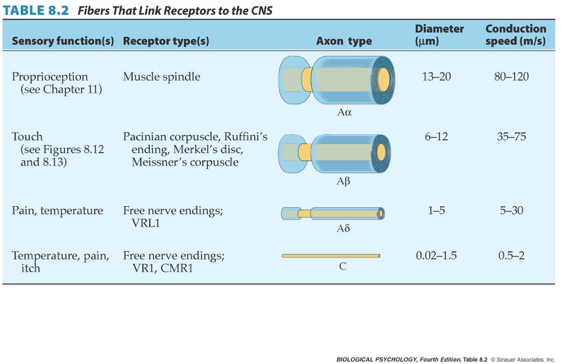
\includegraphics{../include/img/axon-size-speed-tradeoff.jpg}
\end{center}

\subsection{Disorders of movement}\label{disorders-of-movement}

\subsubsection{Parkinson's Disease}\label{parkinsons-disease}

\begin{itemize}
\tightlist
\item
  Slow, absent movement, resting tremor
\item
  Cognitive deficits, depression
\item
  DA Neurons in substantia nigra degenerate
\item
  Treatments

  \begin{itemize}
  \tightlist
  \item
    DA agonists
  \item
    DA agonists linked to impulse control disorders in
    \textasciitilde1/7 patients
    \href{http://doi.org/10.1586/14737175.2016.1158103}{{[}@Ramirez-Zamora2016-rl{]}}
  \item
    Levodopa (L-Dopa), DA precursor
  \end{itemize}
\end{itemize}

\begin{figure}[H]

{\centering 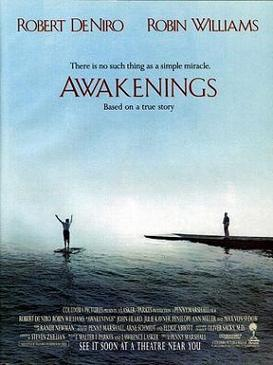
\includegraphics{action_files/mediabag/Awakenings.jpg}

}

\caption{\emph{Awakenings}}

\end{figure}%

\subsubsection{Huntington's Disease}\label{huntingtons-disease}

\begin{figure}[H]

{\centering 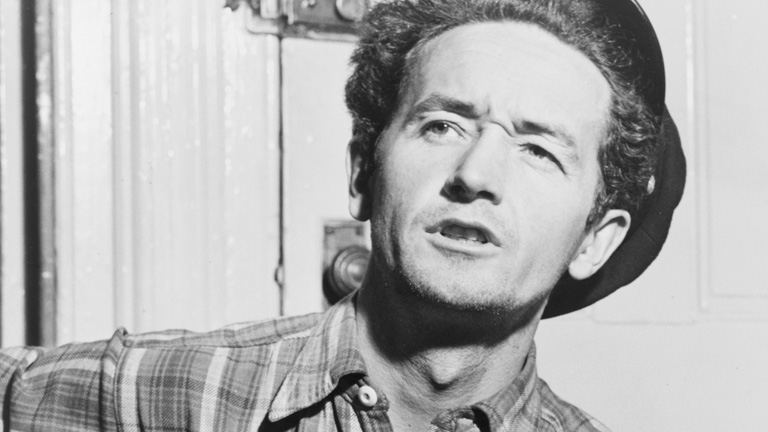
\includegraphics{action_files/mediabag/1000509261001_173382.jpg}

}

\caption{Woody Guthrie}

\end{figure}%

\begin{itemize}
\tightlist
\item
  Formerly Huntington's Chorea

  \begin{itemize}
  \tightlist
  \item
    ``Chorea'' from Greek for ``dance''
  \item
    ``Dance-like'' pattern of involuntary movements
  \end{itemize}
\item
  Cognitive decline
\item
  Genetic + environmental influences
\item
  Disturbance in striatum
\end{itemize}

\paragraph{Prospects}\label{prospects}

\begin{itemize}
\tightlist
\item
  No effective treatment
\item
  But progress in an animal model targeting abnormal protein products
  {[}@Li2019-to{]}
\item
  Clinical trial focused on gene therapy
\end{itemize}

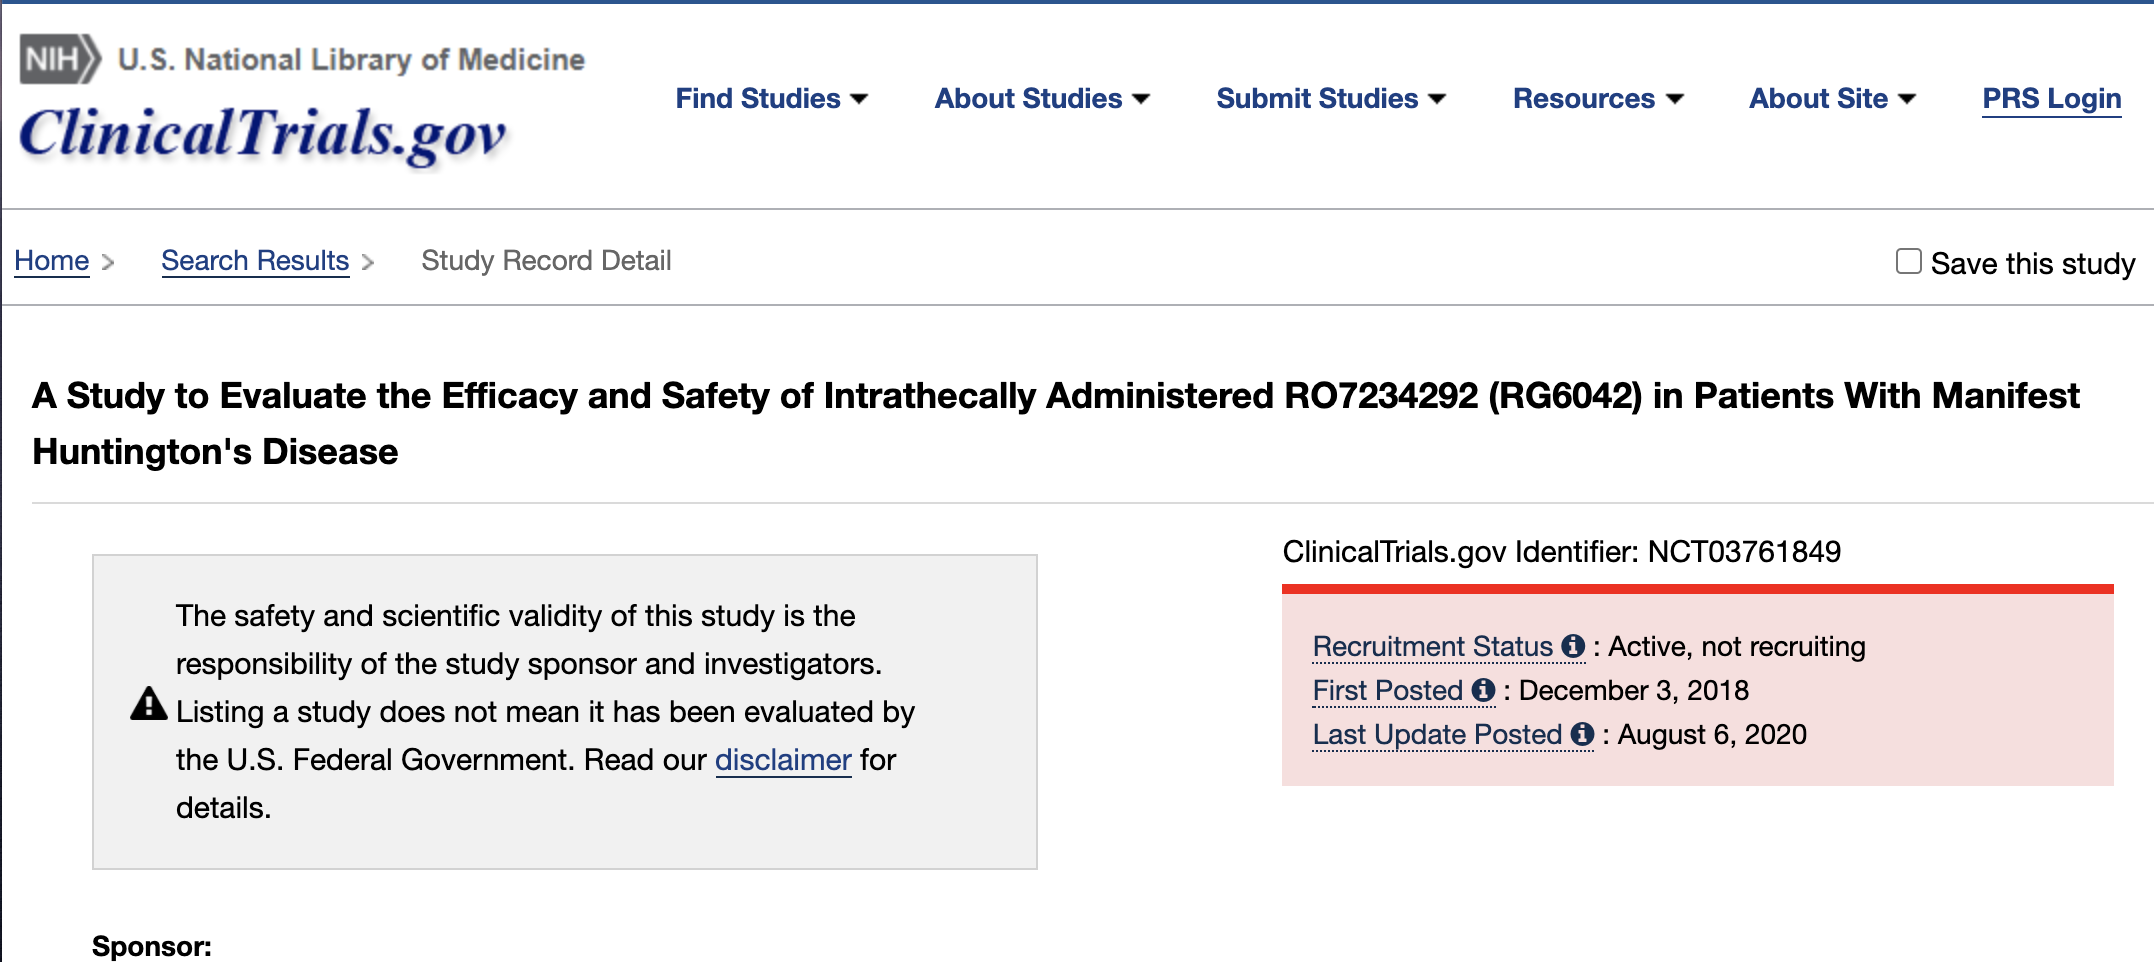
\includegraphics{../include/img/huntingtons-trial.png} - Ended in 2021
due to safety concerns. - {[}@Andrew2023-pq{]}.

\subsection{Summing up}\label{summing-up}

\begin{itemize}
\tightlist
\item
  Control of movement determined by multiple sources
\item
  Cerebral cortex + basal ganglia + cerebellum + spinal circuits
\end{itemize}

\subsubsection{Movement: The ``real'' reason for
brains?}\label{movement-the-real-reason-for-brains}

\subsubsection{What does motor cortex activity
encode?}\label{what-does-motor-cortex-activity-encode}

\begin{itemize}
\tightlist
\item
  Muscle contractions?
\item
  Movement trajectories?
\item
  Representational vs.~dynamical systems views
\end{itemize}

\begin{figure}[H]

{\centering \includegraphics{action_files/mediabag/ne360337.f1.jpeg}

}

\caption{{[}@Shenoy2013-zi{]}. Figure 1. Schematic illustrating the
focus of the representational perspective and of the dynamical systems
perspective. The traditional perspective has concentrated on the
representation or code employed by the motor cortex. For example, does
the motor cortex (upper left panel) code muscle activity (red trace) or
reach velocity (black trace)? Thus, the traditional perspective attempts
to determine the output or controlled parameters of the motor cortex.
The dynamical systems perspective focuses less on the output itself and
more on how that output is created (upper right panel). It attempts to
isolate the basic patterns (blue) from which the final output might be
built. It further attempts to understand the dynamics that produced that
set of patterns and the role of preparatory activity in creating the
right set of patterns for a particular movement. The red trace indicates
the activity of the deltoid versus time during a rightward reach (e.g.,
Churchland et al.~2012). The black trace is the hand velocity for that
same reach; the black trace between the beginning and ending reach
targets is the hand path. The light and dark blue traces (upper right)
illustrate a potential dynamical basis set from which the red trace
might be built.}

\end{figure}%%
\begin{figure}[H]

{\centering \includegraphics{action_files/mediabag/ne360337.f2.jpeg}

}

\caption{{[}@Shenoy2013-zi{]}. Figure 2. Overview of experimental
paradigm, behavioral measurements, muscle measurements, and neural
measurements. (a) Illustration of the instructed-delay task. Monkeys sit
in a primate chair ∼25 cm from a fronto-parallel display. A trial begins
by fixating (eye) and touching (hand) a central target (red filled
square) and holding for a few hundred milliseconds. A peripheral target
(red open square) then appears, cuing the animal about where a movement
must ultimately be made. After a randomized delay period (e.g., 0--1 s)
a go cue is given (e.g., extinction of central fixation and touch
targets) signaling that an arm movement to the peripheral target may
begin. (b) Sample hand measurements and electromyographic (EMG)
recordings for the same trial as in panel a. Top: Horizontal hand
(black) and target (red) positions are plotted. For this experiment, the
target jittered on first appearing and stabilized at the go cue. Bottom:
Hand velocity superimposed on the voltage recorded from the medial
deltoid. (c) Sample reach trajectories and end points in a center-out
two-instructed-speed version of the instructed-delay task. Red and green
traces/symbols correspond to instructed-fast and instructed-slow
conditions. (d) Mean reaction time (RT) plotted versus delay-period
duration. The line shows an exponential fit. (e) Examples of typical
delay-period firing-rate responses in PMd. Mean ± Standard Error firing
rates for four sample neurons are shown. Figure adapted from Churchland
et al.~(2006c).}

\end{figure}%

\subsubsection{\texorpdfstring{Dynamical systems and
\href{https://en.wikipedia.org/wiki/State-space_representation}{state
spaces}}{Dynamical systems and state spaces}}\label{dynamical-systems-and-state-spaces}

\begin{itemize}
\tightlist
\item
  Movement of the limbs and body
\item
  Activity of the muscles
\item
  Activity of neurons in the spinal cord
\item
  Activity of neurons in the brain\ldots{}
\end{itemize}

\begin{figure}[H]

{\centering 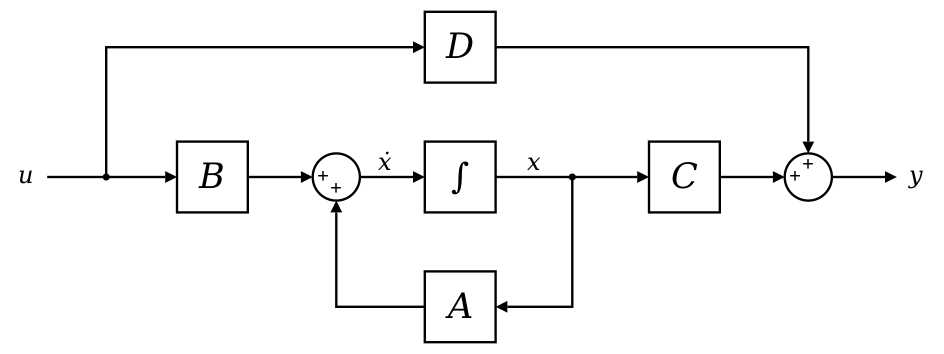
\includegraphics{action_files/mediabag/944px-Typical_State_.png}

}

\caption{Wikipedia}

\end{figure}%

\subsubsection{What does the cerebellum
do?}\label{what-does-the-cerebellum-do}

\begin{itemize}
\tightlist
\item
  Predict future sensory states?
  \href{http://doi.org/10.1038/nrn2332}{{[}@Ito2008-ai{]}}
\end{itemize}

\subsubsection{Systems perspective}\label{systems-perspective}

\begin{itemize}
\tightlist
\item
  Cognitive/affective states
\item
  Nervous system states
\item
  Muscle states
\item
  Actions
\item
  Consequences of actions on world states
\item
  Sensory states
\end{itemize}

\begin{figure}[H]

{\centering 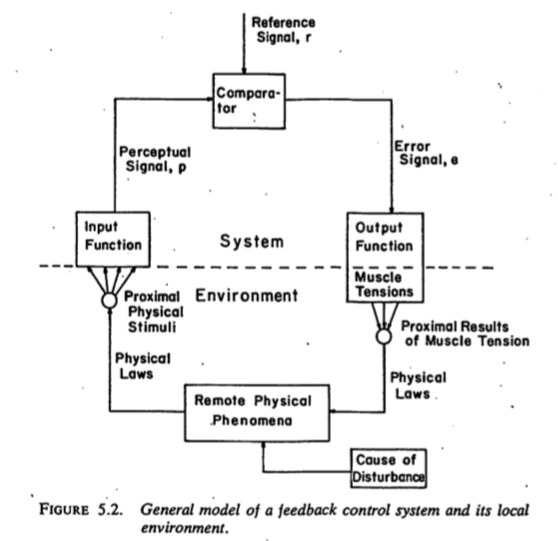
\includegraphics{../include/img/powers-5.2.png}

}

\caption{{[}Figure 5.2 from @Powers1973-zn{]}}

\end{figure}%%
\begin{figure}[H]

{\centering 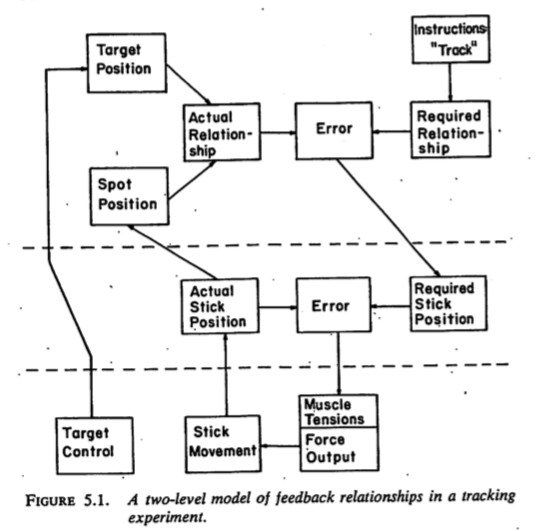
\includegraphics{./include/img/powers-5.1.png}

}

\caption{{[}Figure 5.1 from @Powers1973-zn{]}}

\end{figure}%%
\begin{figure}[H]

{\centering 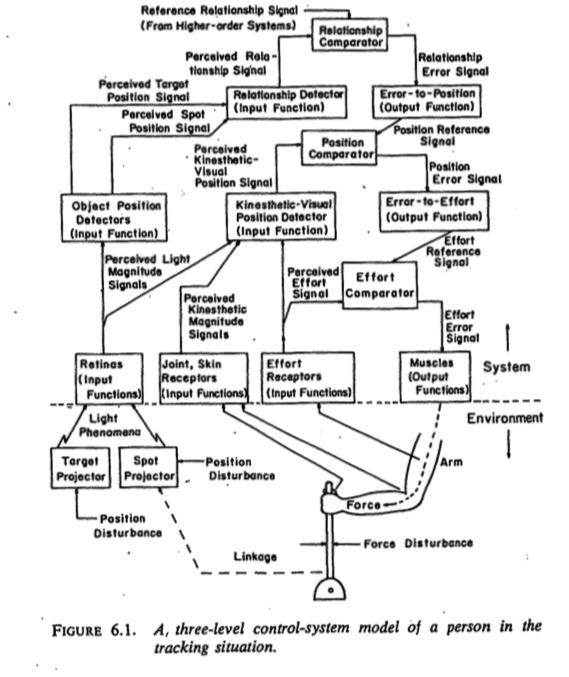
\includegraphics{../include/img/powers-6.1.png}

}

\caption{{[}Figure 6.1 from @Powers1973-zn{]}}

\end{figure}%

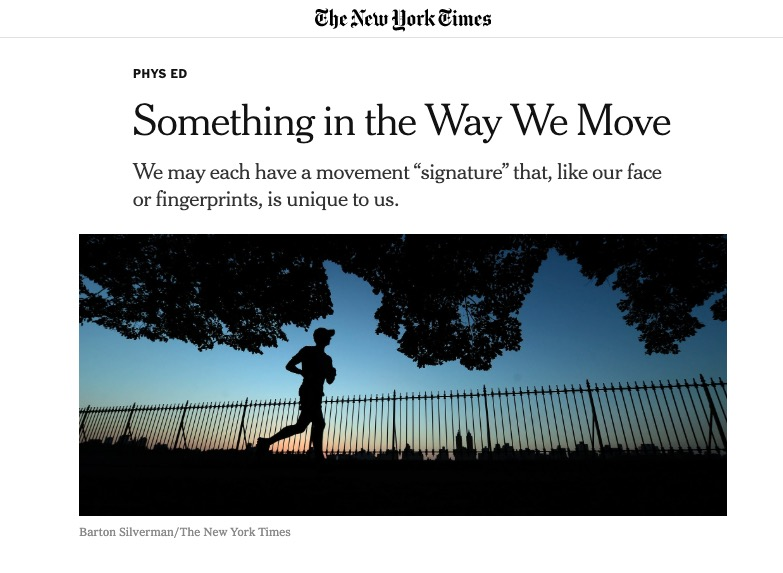
\includegraphics{../include/img/something-in-the-way-we-move.jpg}\{fig-align=
``center''\}

\begin{figure}[H]

{\centering \includegraphics{action_files/mediabag/41593_2018_312_Fig2_.webp}

}

\caption{{[}Figure 2 from @Shine2019-lh{]}. Fig. 2: The low-dimensional
signature across cognitive tasks. a, The procedure used to partition
tPC1 into unique phases: low (blue), rise (red), high (orange), and fall
(light blue). b, Scatter plot comparing the loading of tPC1 (colored
according to the partition defined in a) with a temporal stability
measure (defined by the similarity of the BOLD response at adjacent time
points); we observed a significant positive Pearson's correlation
(r=0.58) between \textbar tPC1\textbar{} and temporal stability (n=1,939
time points), providing heuristic evidence for attractor basins at the
extremes of tPC1 engagement. c, A three-dimensional scatter plot
comparing the first three tPCs; each node represents one time point
(colored according to the phase of tPC1), with time implicitly unfolding
across the embedding space (contiguous points connected by black line).
d, The low-dimensional manifold traversed by the global brain state
across the first three dimensions, with arrows depicting the direction
of flow along the manifold.}

\end{figure}%



\end{document}
